\documentclass[12pt,twoside]{mitthesis-exec}

%%%%%%%%%%%%%%%%%%%%%%%%%%%%%%%%%%%%%%%%%%%%%%%%%%%%%%%%%%%%%%%%%%%%%%%%%%%%%%%%
% PREAMBLE

\usepackage[bitstream-charter]{mathdesign} % Use BT Charter font
\usepackage[T1]{fontenc}                   % Use T1 encoding instead of OT1
\usepackage[utf8]{inputenc}                % Use UTF8 input encoding
\usepackage{microtype}                     % Improve typography
\usepackage{amsmath}                       % AMS Math extensions
\usepackage{booktabs}                      % Improve table spacing
\usepackage{graphicx}                      % Extended graphics capabilities
\usepackage{tocbibind}                     % Include listings in TOC
\usepackage[printonlyused]{acronym} % withpage: for showing page of use
\usepackage{listings}                      % Source code listings
\usepackage{caption}
\usepackage{subcaption}
\usepackage[rgb,table]{xcolor}
\usepackage{url}
\usepackage{soul}
\usepackage{array}
\usepackage{pdfpages}
\usepackage{mathtools}
\usepackage{setspace}
\usepackage{pbox}
\usepackage{tikz}
\usetikzlibrary{calc,shapes,decorations.pathreplacing,positioning}
\usepackage{pgfplots}
\usepackage{siunitx}
\usepackage{multirow}
\usepackage{breqn}

% Specialties for tables
\usepackage{array}
\newcolumntype{L}[1]{>{\raggedright\let\newline\\\arraybackslash\hspace{0pt}}m{#1}}
\newcolumntype{C}[1]{>{\centering\let\newline\\\arraybackslash\hspace{0pt}}m{#1}}
\newcolumntype{R}[1]{>{\raggedleft\let\newline\\\arraybackslash\hspace{0pt}}m{#1}}

\usepackage[breaklinks=true]{hyperref}
\hypersetup{colorlinks=true, linkcolor=black, citecolor=black, urlcolor=black,
  pdftitle={Reactor Agnostic Multi-Group Cross Section Generation for Fine Mesh Deterministic Neutron Transport Simulations},
  pdfauthor={William Robert Dawson Boyd}
}
\pagestyle{plain}

%\usepackage{floatrow}
%\floatsetup[table]{style=plaintop}
%\floatsetup[widefigure]{margins=hangleft}

% Highlights and emphasis boxes from Bryans thesis
\usepackage[framemethod=tikz]{mdframed}
\definecolor{mitred}{rgb}{0.698,0.0314,0.216}
\definecolor{mitgray}{rgb}{0.690,0.694,0.710}
\definecolor{canyellow}{rgb}{0.933, 0.965, 0.424}
\newmdenv[nobreak=false, skipabove=2ex, skipbelow=2ex, innerlinewidth=3pt, innerlinecolor=black, backgroundcolor=mitgray!75, roundcorner=10pt, frametitlerule=true, frametitlerulewidth=2.5pt, frametitlefont=\color{white}\Large\bfseries, frametitlealignment=\centering, frametitlebackgroundcolor=mitred, frametitleaboveskip=2ex, frametitlebelowskip=2ex, innertopmargin=3ex, innerbottommargin=2ex]{highlightsbox}
\newmdenv[nobreak=false, skipabove=2ex, skipbelow=2ex, innerlinewidth=2pt, innerlinecolor=black, backgroundcolor=white, roundcorner=10pt]{emphbox}

% Appendix
\usepackage[toc,page]{appendix}

% Don't reset footnote counter between chapters
\usepackage{chngcntr}
\counterwithout{footnote}{chapter}

% Algorithm constructs
\usepackage[chapter]{algorithm} % Provides algorithm environment
\usepackage{algorithmicx}       % Provides algorithmic block
\usepackage{algpseudocode}      % Option of algorithmicx package
\renewcommand{\thealgorithm}{\thechapter-\arabic{algorithm}}
\newcommand\Algphase[1]{%
\vspace*{-.7\baselineskip}\Statex\hspace*{\dimexpr-\algorithmicindent-2pt\relax}\rule{\columnwidth}{0.4pt}%
\Statex\hspace*{-\algorithmicindent}{#1}%
\vspace*{-.7\baselineskip}\Statex\hspace*{\dimexpr-\algorithmicindent-2pt\relax}\rule{\columnwidth}{0.4pt}%
}
\newcommand{\algrule}[1][.4pt]{\par\vskip.5\baselineskip\hrule height #1\par\vskip.5\baselineskip}

% Configure captions
\captionsetup{labelfont=bf, labelsep=colon}
\captionsetup[algorithm]{labelfont=bf, labelsep=colon}

% Use Latin Modern for typewriter fonts
\renewcommand{\ttdefault}{lmtt}

% Add \unit macro
\newcommand{\unit}[1]{\ensuremath{\, \mathrm{#1}}}

\definecolor{gray}{rgb}{0.4,0.4,0.4}
\definecolor{darkblue}{rgb}{0.0,0.0,0.6}
\definecolor{cyan}{rgb}{0.0,0.6,0.6}
\lstset{
  basicstyle=\footnotesize\ttfamily,
  columns=fullflexible,
  showstringspaces=false,
  commentstyle=\color{gray}\upshape,
  frame=single,
  xleftmargin=0.55in
}

\lstdefinelanguage{XML}
{
  morestring=[b]",
  morestring=[s]{>}{<},
  morecomment=[s]{<?}{?>},
  morecomment=[s]{<!--}{-->},
  stringstyle=\color{black},
  identifierstyle=\color{darkblue},
  keywordstyle=\color{cyan},
  morekeywords={}
}

\setcounter{secnumdepth}{4}
\setcounter{tocdepth}{3}

\renewcommand{\contentsname}{Table of Contents}
\renewcommand{\bibname}{References}

\makeatletter \renewcommand\thealgorithm{\arabic{algorithm}} \@addtoreset{algorithm}{chapter} \makeatother

\begin{document}

%%%%%%%%%%%%%%%%%%%%%%%%%%%%%%%%%%%%%%%%%%%%%%%%%%%%%%%%%%%%%%%%%%%%%%%%%%%%%%%%
% TITLE PAGE

\title{EXECUTIVE SUMMARY \\~\\ Reactor Agnostic Multi-Group Cross Section Generation for Fine Mesh Deterministic Neutron Transport Simulations}

\author{William Robert Dawson Boyd III}
\prevdegrees{B.S., Georgia Institute of Technology (2010) \\
             M.S., Massachusetts Institute of Technology (2014)}
\department{Department of Nuclear Science and Engineering}
\degree{Doctor of Philosophy in Nuclear Science and Engineering}

\degreemonth{February}
\degreeyear{2017}
\thesisdate{November 4, 2016}

\supervisor{Benoit Forget}{Associate Professor of Nuclear Science and Engineering}
\reader{Kord S. Smith}{KEPCO Professor of the Practice of Nuclear Science and Engineering}
\chairman{Emilio Bagglietto}{Associate Professor of Nuclear Science and Engineering}


%%%%%%%%%%%%%%%%%%%%%%%%%%%%%%%%%%%%%%%%%%%%%%%%%%%%%%%%%%%%%%%%%%%%%%%%%%%%%%%%
%%%%%%%%%%%%%%%%%%%%%%%%%%%%%%%%%%%%%%%%%%%%%%%%%%%%%%%%%%%%%%%%%%%%%%%%%%%%%%%%
% ABSTRACT

\setcounter{savepage}{\thepage}

\begin{abstractpage}

The development of high fidelity multi-group neutron transport-based simulation tools for full core Light Water Reactor (LWR) analysis has been a long-standing goal of the reactor physics community. While direct transport simulations have previously been far too computationally expensive, advances in computer hardware have allowed large scale simulations to become feasible. Therefore, many have focused on developing full core neutron transport solvers that do not incorporate the approximations and assumptions of traditional nodal diffusion solvers. 

Due to the computational expense of direct full core 3D deterministic neutron transport methods, many have focused on 2D/1D methods which solve 3D problems as a coupled system of radial and axial transport problems. However, the coupling of radial and axial problems also introduces approximations. Instead, the work in this thesis focuses on explicitly solving the 3D deterministic neutron transport equations with the Method of Characteristics (MOC).

MOC has been widely used for 2D lattice physics calculations due to its ability to accurately and efficiently simulate reactor physics problems with explicit geometric detail. The work in this thesis strives to overcome the significant computational cost of solving the 3D MOC equations by implementing efficient track generation, axially extruded ray tracing, Coarse Mesh Finite Difference (CMFD) acceleration, linear track-based source approximations, and scalable domain decomposition. 

Additionally, significant attention has been be given to complications that arise in full core simulations with transport-corrected cross-sections. The convergence behavior of transport methods is analyzed, leading to a new strategy for stabilizing the source iteration scheme for neutron transport simulations. The methods are incorporated into the OpenMOC reactor physics code and simulation results are presented for the full core BEAVRS LWR benchmark. Parameter refinement studies and comparisons with reference OpenMC Monte Carlo solutions show that converged full core 3D MOC simulations are feasible on modern supercomputers for the first time.

%However, 3D full core LWR simulations present significant challenges due to greatly increased computational cost.

%The Method of Characteristics (MOC) has seen wide interest in reactor physics because of its accuracy and efficiency in computing lattice physics problems. While most of its use has been in solving 2D problems, there has been recent interest in extending MOC to 3D in order to more accurately calculate 3D power distributions in LWRs. While the method is naturally extensible to 3D, it presents significant computational difficulties. Methods will be presented which mitigate the computational difficulties of 3D MOC by using domain decomposition, efficient track generation, axially extruded ray tracing, CMFD acceleration, and a linear source approximation. Significant attention will be given to complications that arise in full core simulations. 3D MOC results will be presented for the full core simulation of the BEAVRS benchmark, showing that 3D MOC can be a viable tool for anal

\end{abstractpage}

\singlespacing 

%%%%%%%%%%%%%%%%%%%%%%%%%%%%%%%%%%%%%%%%%%%%%%%%%%%%%%%%%%%%%%%%%%%%%%%%%%%%%%%%
\section*{Introduction}

%%%%%%%%%%%%%%%%%%%%%%%%%%%%%%%%%%%%%%%
\subsection*{Background and Motivation}

The development and deployment of neutron physics simulations is governed by tradeoffs between accuracy and speed. High-fidelity simulations are \textit{accurate} and \textit{flexible} but require significant computational resources, while the \textit{approximations} made by low-fidelity methods reduce the number of variables which greatly improves the \textit{time-to-solution}. As a result, it is common to employ a mix of high- and low-fidelity tools for reactor analysis -- for example, high-fidelity tools are frequently used to inform and benchmark low-fidelity models for use within a narrow envelope of design parameters. This thesis develops a new approach within the same vein by employing continuous energy Monte Carlo (MC) neutron transport simulations to generate accurate multi-group cross sections (MGXS) for computationally efficient deterministic transport methods.

%\textbf{This thesis is motivated by the desire to obtain Monte Carlo-quality solutions with computationally efficient deterministic neutron transport methods.}

This thesis investigates the use of Monte Carlo methods to generate MGXS, such as the U-235 fission MGXS illustrated in Fig.~\ref{fig:u235-sigf}, for whole-core deterministic reactor analysis. Monte Carlo presents a natural approach to replace engineering prescriptions to approximate the flux with a stochastic approximation of the exact flux. The advantage of a MC-based approach is that all of the relevant physics modeled in MC may be directly embedded into MGXS. This improvement in accuracy comes at the computational expense of converging group constant tallies to acceptably low uncertainties. MC methods have increasingly been used to generate few group constants for coarse mesh diffusion, most notably by the Serpent MC code~\cite{serpent2013manual}. However, there exist few rigorous and comprehensive analyses of MGXS generation for heterogeneous fine mesh deterministic transport methods~\cite{redmond1997multigroup,cai2014condensation,nelson2014improved}. \textbf{This thesis develops and evaluates MC-based methods to generate MGXS for fine mesh deterministic neutron transport codes.}

\begin{figure}[h!]
\centering
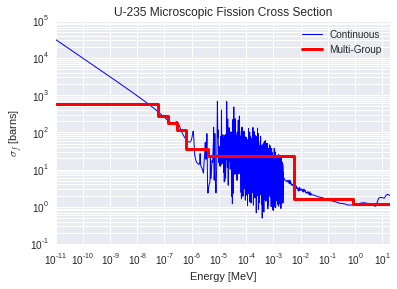
\includegraphics[width=0.75\linewidth]{figures/intro/u235-ce-mg-xs}
\caption[U-235 continuous energy and multi-group fission cross section]{U-235 continuous energy and 16-group fission cross section.}
\label{fig:u235-sigf}
\end{figure}

In addition, MC-based MGXS generation methods to date have retained the multi-level geometric framework illustrated in Fig.~\ref{fig:multi-level-flow-chart} to tabulate MGXS for individual reactor components -- such as infinite fuel pins and/or assemblies -- for subsequent use in whole-core multi-group calculations. The multi-level approach is inspired by legacy MGXS generation techniques which apply high-fidelity models of the energy self-shielding physics to low-fidelity geometric models of unique core components. The complexity of the energy treatment is then reduced at each level as larger and more complex geometric models are considered. \textbf{This thesis abandons the multi-level framework in place of a whole-core MC calculation which simultaneously accounts for all energy and spatial self-shielding effects in a single step.}

\begin{figure}[h!]
\centering
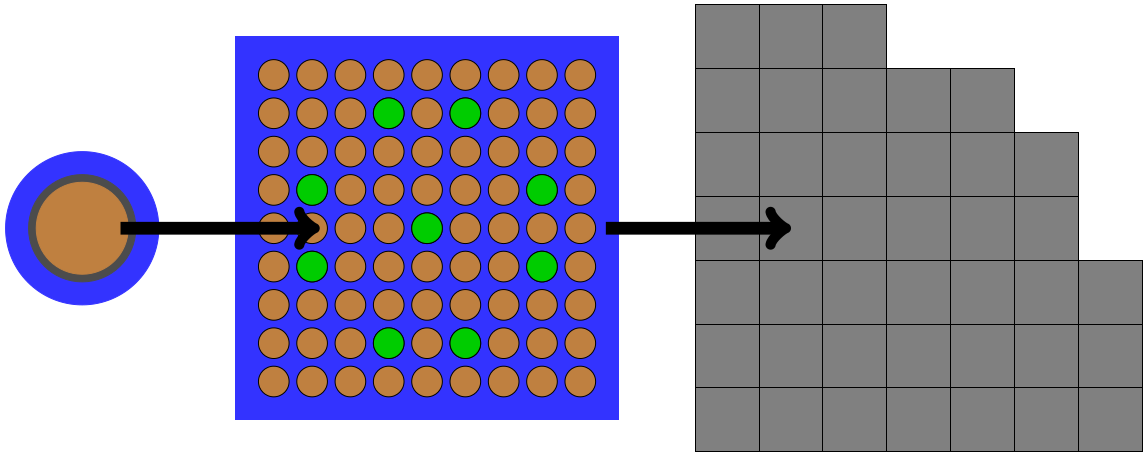
\includegraphics[width=0.9\linewidth]{figures/intro/multi-step-flow-chart}
\caption[Multi-level approach to reactor analysis]{Current multi-level framework for reactor analysis.}
\label{fig:multi-level-flow-chart}
\end{figure}

This thesis uses statistical clustering algorithms to accelerate whole-core MC calculations
which simultaneously model all energy and spatial self-shielding effects for fine mesh MGXS generation in a single step.

\clearpage

%%%%%%%%%%%%%%%%%%%%%%%%
\subsection*{Objectives}

The subject matter of this thesis is organized along two main themes:

\begin{itemize}
\item \textbf{\textit{Approximation Error}} -- Quantify and diagnose approximation error in MGXS generated from MC methods for simple heterogeneous benchmark problems.
\item \textbf{\textit{Statistical Clustering}} -- Develop statistical clustering methods to accelerate the convergence of MGXS on heterogeneous MC tally meshes.
\end{itemize}

\clearpage

%%%%%%%%%%%%%%%%%%%%%%%%%%%%%%%%%%%%%%%%%%%%%%%%%%%%%%%%%%%%%%%%%%%%%%%%%%%%%%%%
\section*{Software Infrastructure: A Simulation Triad}

This thesis investigates Monte Carlo as a means to generate multi-group cross sections for fine mesh transport codes. This work required the development of a ``simulation triad'' encompassing three primary codes as illustrated in Fig.~\ref{fig:simulation-triad}. First, the OpenMC Monte Carlo code~\cite{romano2013openmc} was utilized to generate multi-group cross sections. Second, the MGXS were used by the OpenMOC code~\cite{boyd2014openmoc} for deterministic multi-group transport calculations. Finally, the OpenCG library~\cite{boyd2015opencg} enabled the processing and transfer of tally data on combinatorial geometry (CG) meshes between OpenMC and OpenMOC. The following sections summarize the author's contributions to each component code in the simulation triad to support the objectives of this thesis.

\begin{figure}[h!]
  \centering
  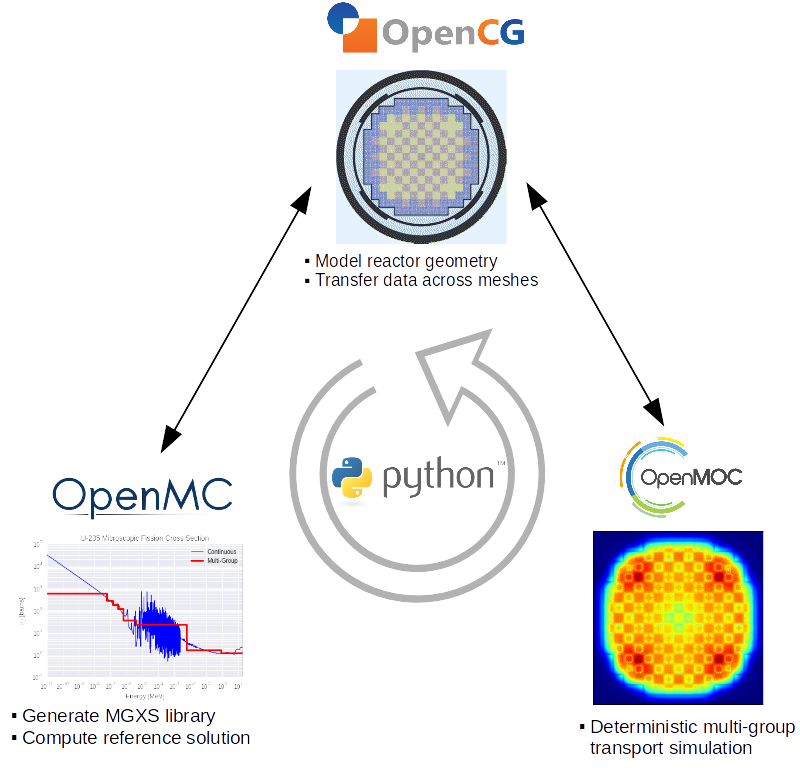
\includegraphics[width=\linewidth]{figures/workflow/triad/simulation-triad}
\caption[A simulation triad of OpenMC, OpenMOC and OpenCG]{A simulation triad consisting of the OpenMC, OpenMOC and OpenCG codes ``glued'' together with Python formed the foundation for this thesis research.}
\label{fig:simulation-triad}
\end{figure}

%%%%%%%%%%%%%%%%%%%%
\subsection*{OpenMC}

The OpenMC code is a continuous energy Monte Carlo neutron transport code~\cite{romano2013openmc} with support for general constructive solid geometry models. This thesis designed and implemented a fully-featured OpenMC Python API to enable the processing of large tally datasets to generate MGXS. In addition, a distributed cell tally algorithm~\cite{lax2014distribcell} was implemented in OpenMC to compute MGXS across repeated fuel pin cells in reactor core geometries. Finally, an option for isotropic in lab scattering was implemented and used to generate MGXS. The isotropic scattering feature enabled ``apples-to-apples'' comparisons between the reference eigenvalues and reaction rates produced by OpenMC and those computed from isotropic multi-group calculations with OpenMOC. In total, the author contributed over 20,000 lines of Python and 2,000 lines of Fortran code to the open source release version of OpenMC to support this work.

%%%%%%%%%%%%%%%%%%%%%
\subsection*{OpenMOC}

The OpenMOC code is a multi-group neutron transport code implementing the deterministic Method of Characteristics (MOC)~\cite{boyd2014openmoc}. The OpenMOC code is capable of performing 2D MOC neutron transport calculations for LWR core configurations. The \texttt{openmoc.materialize} Python module was implemented to automate the loading MGXS data into OpenMOC \texttt{Material} objects. The module is designed to support the large MGXS libraries generated by OpenMC. In addition, a new module was implemented  to interface with the OpenCG region differentiation algorithm, which constructed ``clustered geometries'' for OpenMOC. Finally, a scheme to compute SuPerHomog\'{e}n\'{e}isation (SPH) factors to ensure reaction rate consistency with OpenMC was implemented in OpenMOC. In total, the author contributed over 15,000 lines of C++ and nearly 20,000 lines of Python code to the open source release version of OpenMOC to support this work.

%%%%%%%%%%%%%%%%%%%%
\subsection*{OpenCG}

A new combinatorial goemetry (CG) Python library called OpenCG~\cite{boyd2015opencg} was developed to accelerate the building of complicated reactor geometries and facilitate large scale data processing. The simulation triad shown in Fig.~\ref{fig:simulation-triad} includes ``compatibility modules'' which export OpenCG geometries to OpenMC and OpenMOC. Two novel algorithms known as Local Neighbor Symmetry (LNS) and region differentiation were developed in OpenCG to enable the spatial homogenization methodology introduced in this thesis. First, the LNS algorithm is analogous to the geometric templates used in lattice physics codes such as CASMO~\cite{edenius1995casmo} to identify fuel pins which have similar MGXS. The LNS algorithm performs a systematic analysis of a geometry to identify neighbor cells, or pairs of cells which are adjacent to one another. Second, the region differentiation algorithm was developed to efficiently and systematically construct geometries to reflect the assignment of MGXS to arbitrary ``clusters'' of fuel pins for the spatial homogenization methodology. The differentiated geometries are then exported to OpenMOC for deterministic neutron transport calculations. In total, the author contributed over 10,000 lines of Python code in OpenCG to support this work.

\clearpage

%%%%%%%%%%%%%%%%%%%%%%%%%%%%%%%%%%%%%%%%%%%%%%%%%%%%%%%%%%%%%%%%%%%%%%%%%%%%%%%%%
%\section*{Angular-Dependent MGXS and SPH Factors}
%
%%%%%%%%%%%%%%%%%%%%%%%%%%%%%%%%%%%%%%%%%%%%%%
%\subsection*{Flux Separability Approximation}
%
%\begin{dmath}
%\label{eqn:sigt-flux-separable}
%\Sigma_{t,g}(\mathbf{r}) = \frac{\int\displaylimits_{E_{g}}^{E_{g-1}} \Sigma_{t}(\mathbf{r},E)\psi(\mathbf{r},\mathbf{\Omega},\mathrm{d}E)}{\psi_{g}(\mathbf{r},\mathbf{\Omega})} \approx \frac{\int\displaylimits_{E_{g}}^{E_{g-1}} \Sigma_{t}(\mathbf{r},E)\phi(\mathbf{r},E)}{\phi_{g}(\mathbf{r})}
%\end{dmath}
%
%\clearpage
%
%%%%%%%%%%%%%%%%%%%%%%%%%%%%%%%%%%%%%%%%%%%
%\subsection*{Energy-Dependent Flux Errors}
%
%\begin{figure}[h!]
%\centering
%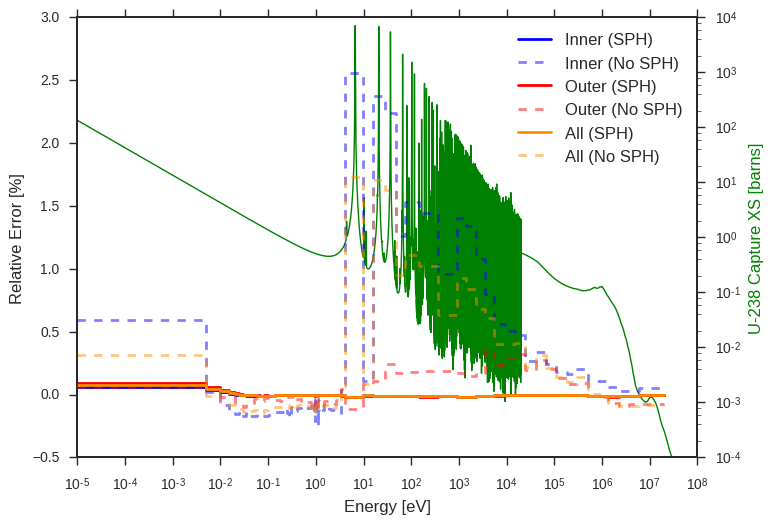
\includegraphics[width=\linewidth]{figures/sph/pin-cell/rel-err-inner-outer}
%\caption[Flux relative error by energy group with SPH]{The energy-dependent relative error of the 70-group OpenMOC scalar flux with respect to the OpenMC flux in a fuel pin for the innermost, outermost and all FSRs.}
%\label{fig:rel-err-energy}
%\end{figure}
%
%\clearpage

%%%%%%%%%%%%%%%%%%%%%%%%%%%%%%%%%%%%%
%\subsection*{Angular-Dependent MGXS}
%
%\begin{figure}[h]
%\begin{subfigure}{.5\textwidth}
%  \centering
%  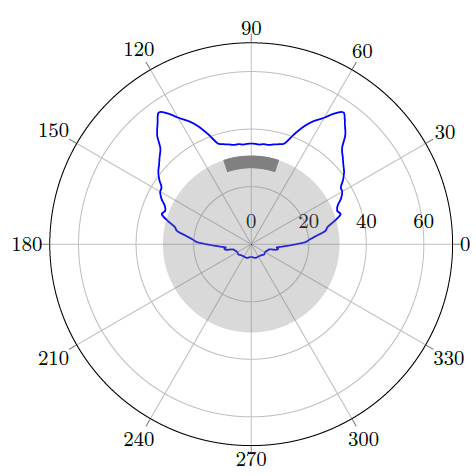
\includegraphics[width=\linewidth]{figures/sph/batman-1}
%  \caption{}
%  \label{fig:batman-plots-a}
%\end{subfigure}
%\begin{subfigure}{.5\textwidth}
%  \centering
%  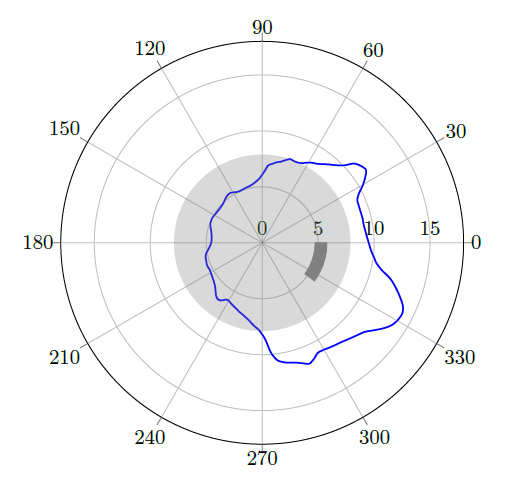
\includegraphics[width=\linewidth]{figures/sph/batman-2}
%  \caption{}
%  \label{fig:batman-plots-b}
%\end{subfigure}
%\caption[Angular-dependent capture MGXS]{Angular-dependent capture MGXS for the 6.67 eV resonance group as a function of azimuthal angle for two different FSRs. The radial axis is given in units of barns and the azimuthal axis in units of degrees. \textit{Image courtesy of N. Gibson~\cite{gibson2016thesis}.}}
%\label{fig:batman-plots}
%\end{figure}
%
%\clearpage
%
%%%%%%%%%%%%%%%%%%%%%%%%%%%%%%%%%%%%%%%%%%%%%%%%%%%
%\subsection*{SuPerHomog\'{e}n\'{e}isation Factors}
%
%-SPH factors were first proposed by H\'{e}bert~\cite{hebert1993consistent} to preserve reaction rates during energy condensation and spatial homogenization \\
%-SPH factor algorithm requires knowledge of a reference source that is used in a multi-group fixed source solver to derive multiplicative factors that adjust the total MGXS to force neutron balance \\
%
%\begin{dmath}
%\label{eqn:sph-transport-eqn-iterate}
%\mathbf{\Omega} \cdot \nabla \psi_{g}^{(n)}(\mathbf{r},\mathbf{\Omega}) + \mu_{k,g}^{(n-1)}\Sigma_{t,k,g}\psi_{g}^{(n)}(\mathbf{r},\mathbf{\Omega}) = Q_{k,g}(\mathbf{\Omega})
%\end{dmath}
%
%\begin{dmath}
%\label{eqn:sph-update-sigt}
%\Sigma_{t,k,g}^{(n)} = \mu_{k,g}^{(n-1)}\Sigma_{t,k,g}^{(0)}
%\end{dmath}
%
%\begin{algorithm}[h]
%\caption{SPH Factor Algorithm}
%\label{alg:sph}
%\begin{algorithmic}[1]
%%  \State Initialize MGXS from MC tallies
%%  \State Compute neutron source from MC flux and MGXS
%  \State Initialize SPH factors to unity
%  \While{SPH factors are not converged}
%    \State Update MGXS with SPH factors \Comment{Eqn.~\ref{eqn:sph-update-sigt}}
%    \State Solve fixed source transport problem \Comment{Eqn.~\ref{eqn:sph-transport-eqn-iterate}}
%    \State Compute new SPH factors
%  \EndWhile
%  \State Compute final MGXS with SPH factors \Comment{Eqn.~\ref{eqn:sph-update-sigt}}
%\end{algorithmic}
%\end{algorithm}
%
%\begin{table}[h!]
%  \centering
%  \caption[Eigenvalues with and without SPH factors for a fuel pin]{The impact of SPH factors on the eigenvalue bias $\Delta\rho$ with varying energy group structures for a fuel pin.}  
%  \label{table:sph-keff}
%  \vspace{6pt}
%  \begin{tabular}{c S[table-format=6.1] S[table-format=6.1]}
%  \toprule
%  & \multicolumn{2}{c}{{\bf $\boldsymbol{\Delta\rho}$ [pcm]}} \\
%  \cline{2-3}
%  \multirow{-2}{*}{{\bf \# Groups}} &
%  \multicolumn{1}{c}{{\bf Without SPH}} &
%  \multicolumn{1}{c}{{\bf With SPH}} \\
%  \midrule
%1 & 66 & -14 \\
%2 & 34 & -6\\
%4 & -57 & 1 \\
%8 & -102 & 2 \\
%16 & -111 & 4 \\
%25 & -182 & -1 \\
%40 & -202 & 2 \\
%70 & -211 & -3 \\
%  \bottomrule
%\end{tabular}
%\end{table}
%
%\clearpage

%%%%%%%%%%%%%%%%%%%%%%%%%%%%%%%%%%%%%%%%%
\section*{Spatial Homogenization Schemes}

%%%%%%%%%%%%%%%%%%%%%%%%%%%%%%%%%%%%%%%%%%%%%%%%%%%
\subsection*{Track Density-Weighted Homogenization}

\begin{equation}
\label{eqn:imgxs-set}
\mathbb{S}_{m} = \left\{1 \le k \le K: S(k) = m\right\}
\end{equation}

LNS homogenization computes a single set of MGXS for the fuel pin instances in each set $k \in \mathbb{S}_{m}$ classified by the LNS algorithm. This is equivalent to a specialization of Eqn.~\ref{eqn:imgxs-micro} with track density-weighted averages of the reaction rates and flux tallies in each pin instance:

\begin{equation}
\label{eqn:imgxs-micro}
\hat{\sigma}_{x,i,m,g} = \frac{\displaystyle\sum\limits_{k=1}^{K}\mathbb{1}_{\mathbb{S}_{m}}(k) \langle \sigma_{x,i}, \psi \rangle_{k,g}^{t\ell}}{\displaystyle\sum\limits_{k=1}^{K}\mathbb{1}_{\mathbb{S}_{m}}(k) \langle \psi \rangle_{k,g}^{t\ell}}
\end{equation}

\begin{figure}[h!]
\centering
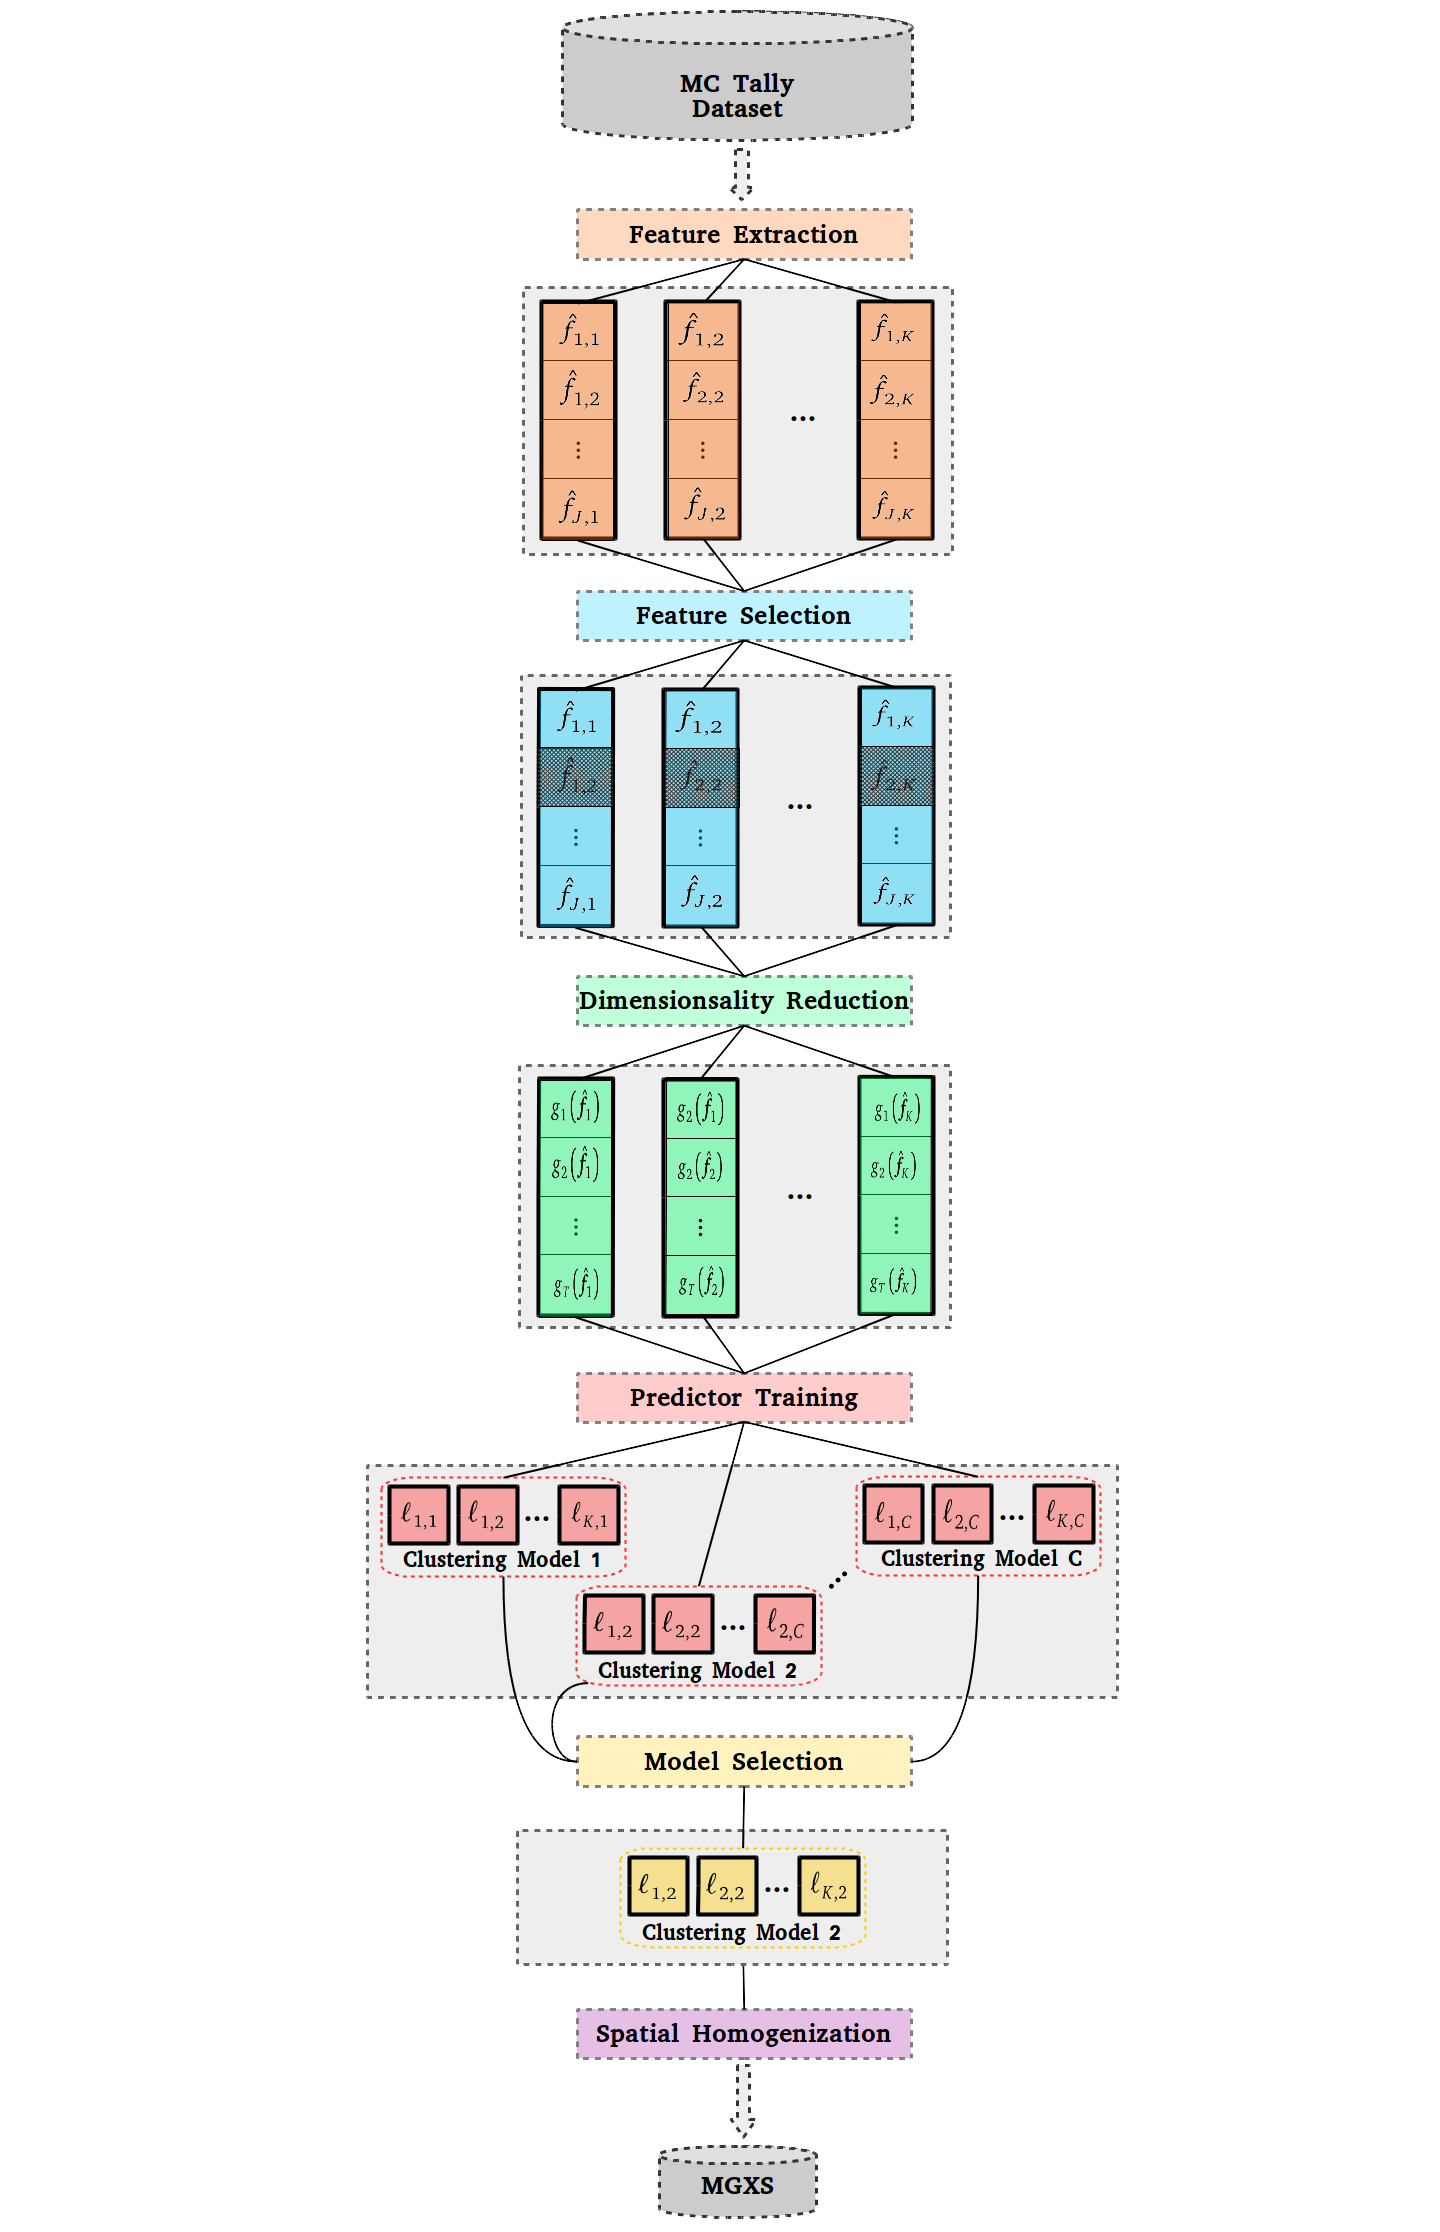
\includegraphics[width=0.9\linewidth]{figures/unsupervised/features/engineering/flow-chart}
\vspace{2mm}
\caption[\textit{i}MGXS flow chart]{The \textit{i}MGXS data processing pipeline.}
\label{fig:imgxs-flow-chart}
\end{figure}

\begin{figure}[h!]
\centering
\begin{subfigure}{0.45\textwidth}
  \centering
  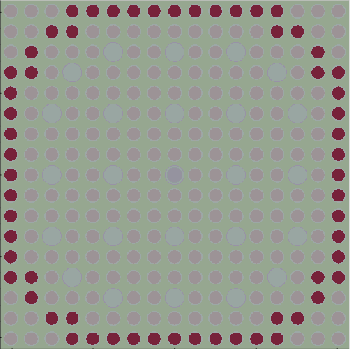
\includegraphics[width=0.9\linewidth]{figures/unsupervised/features/assm-16/u238-capt/mean-pcm/geometry-2}
  \caption{}
  \label{fig:chap10-capt-mean-pcm-geom-2}
\end{subfigure}%
\begin{subfigure}{0.45\textwidth}
  \centering
  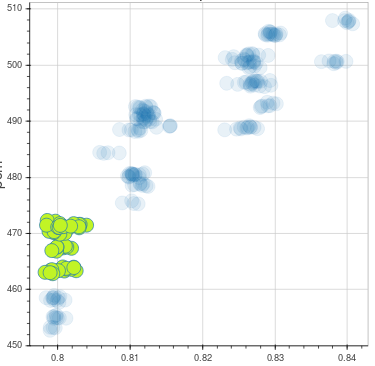
\includegraphics[width=0.9\linewidth]{figures/unsupervised/features/assm-16/u238-capt/mean-pcm/mgxs-2}
  \caption{}
  \label{fig:chap10-capt-mean-pcm-mgxs-2}
\end{subfigure}
\begin{subfigure}{0.45\textwidth}
  \centering
  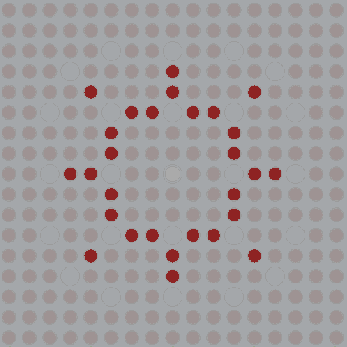
\includegraphics[width=0.9\linewidth]{figures/unsupervised/features/assm-16/u238-capt/mean-pcm/geometry-3}
  \caption{}
  \label{fig:chap10-capt-mean-pcm-geom-3}
\end{subfigure}%
\begin{subfigure}{0.45\textwidth}
  \centering
  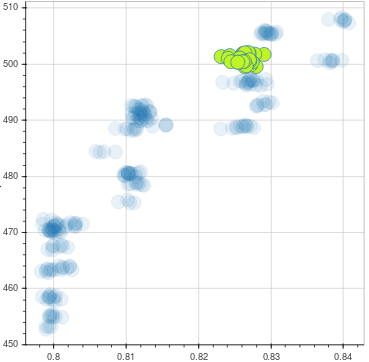
\includegraphics[width=0.9\linewidth]{figures/unsupervised/features/assm-16/u238-capt/mean-pcm/mgxs-3}
  \caption{}
  \label{fig:chap10-capt-mean-pcm-mgxs-3}
\end{subfigure}
\caption[Clustering of U-238 capture MGXS fractional reactivities]{Scatter plots of the pin-wise U-238 capture MGXS means ($x$) and fractional reactivities ($y$) for a 1.6\% enriched fuel assembly.}
\label{fig:capt-mean-std}
\end{figure}

\clearpage

%%%%%%%%%%%%%%%%%%%%%%%%%%%
\section*{Model Validation}

%%%%%%%%%%%%%%%%%%%%%%%%%%%%%%%%%%%%%%%%%%
\subsection*{Heterogeneous PWR Benchmarks}

-construction of six heterogeneous benchmarks from BEAVRS~\cite{horelik2013beavrs} \\

\clearpage

\begin{figure}[h!]
\centering
\begin{subfigure}{0.47\textwidth}
  \centering
  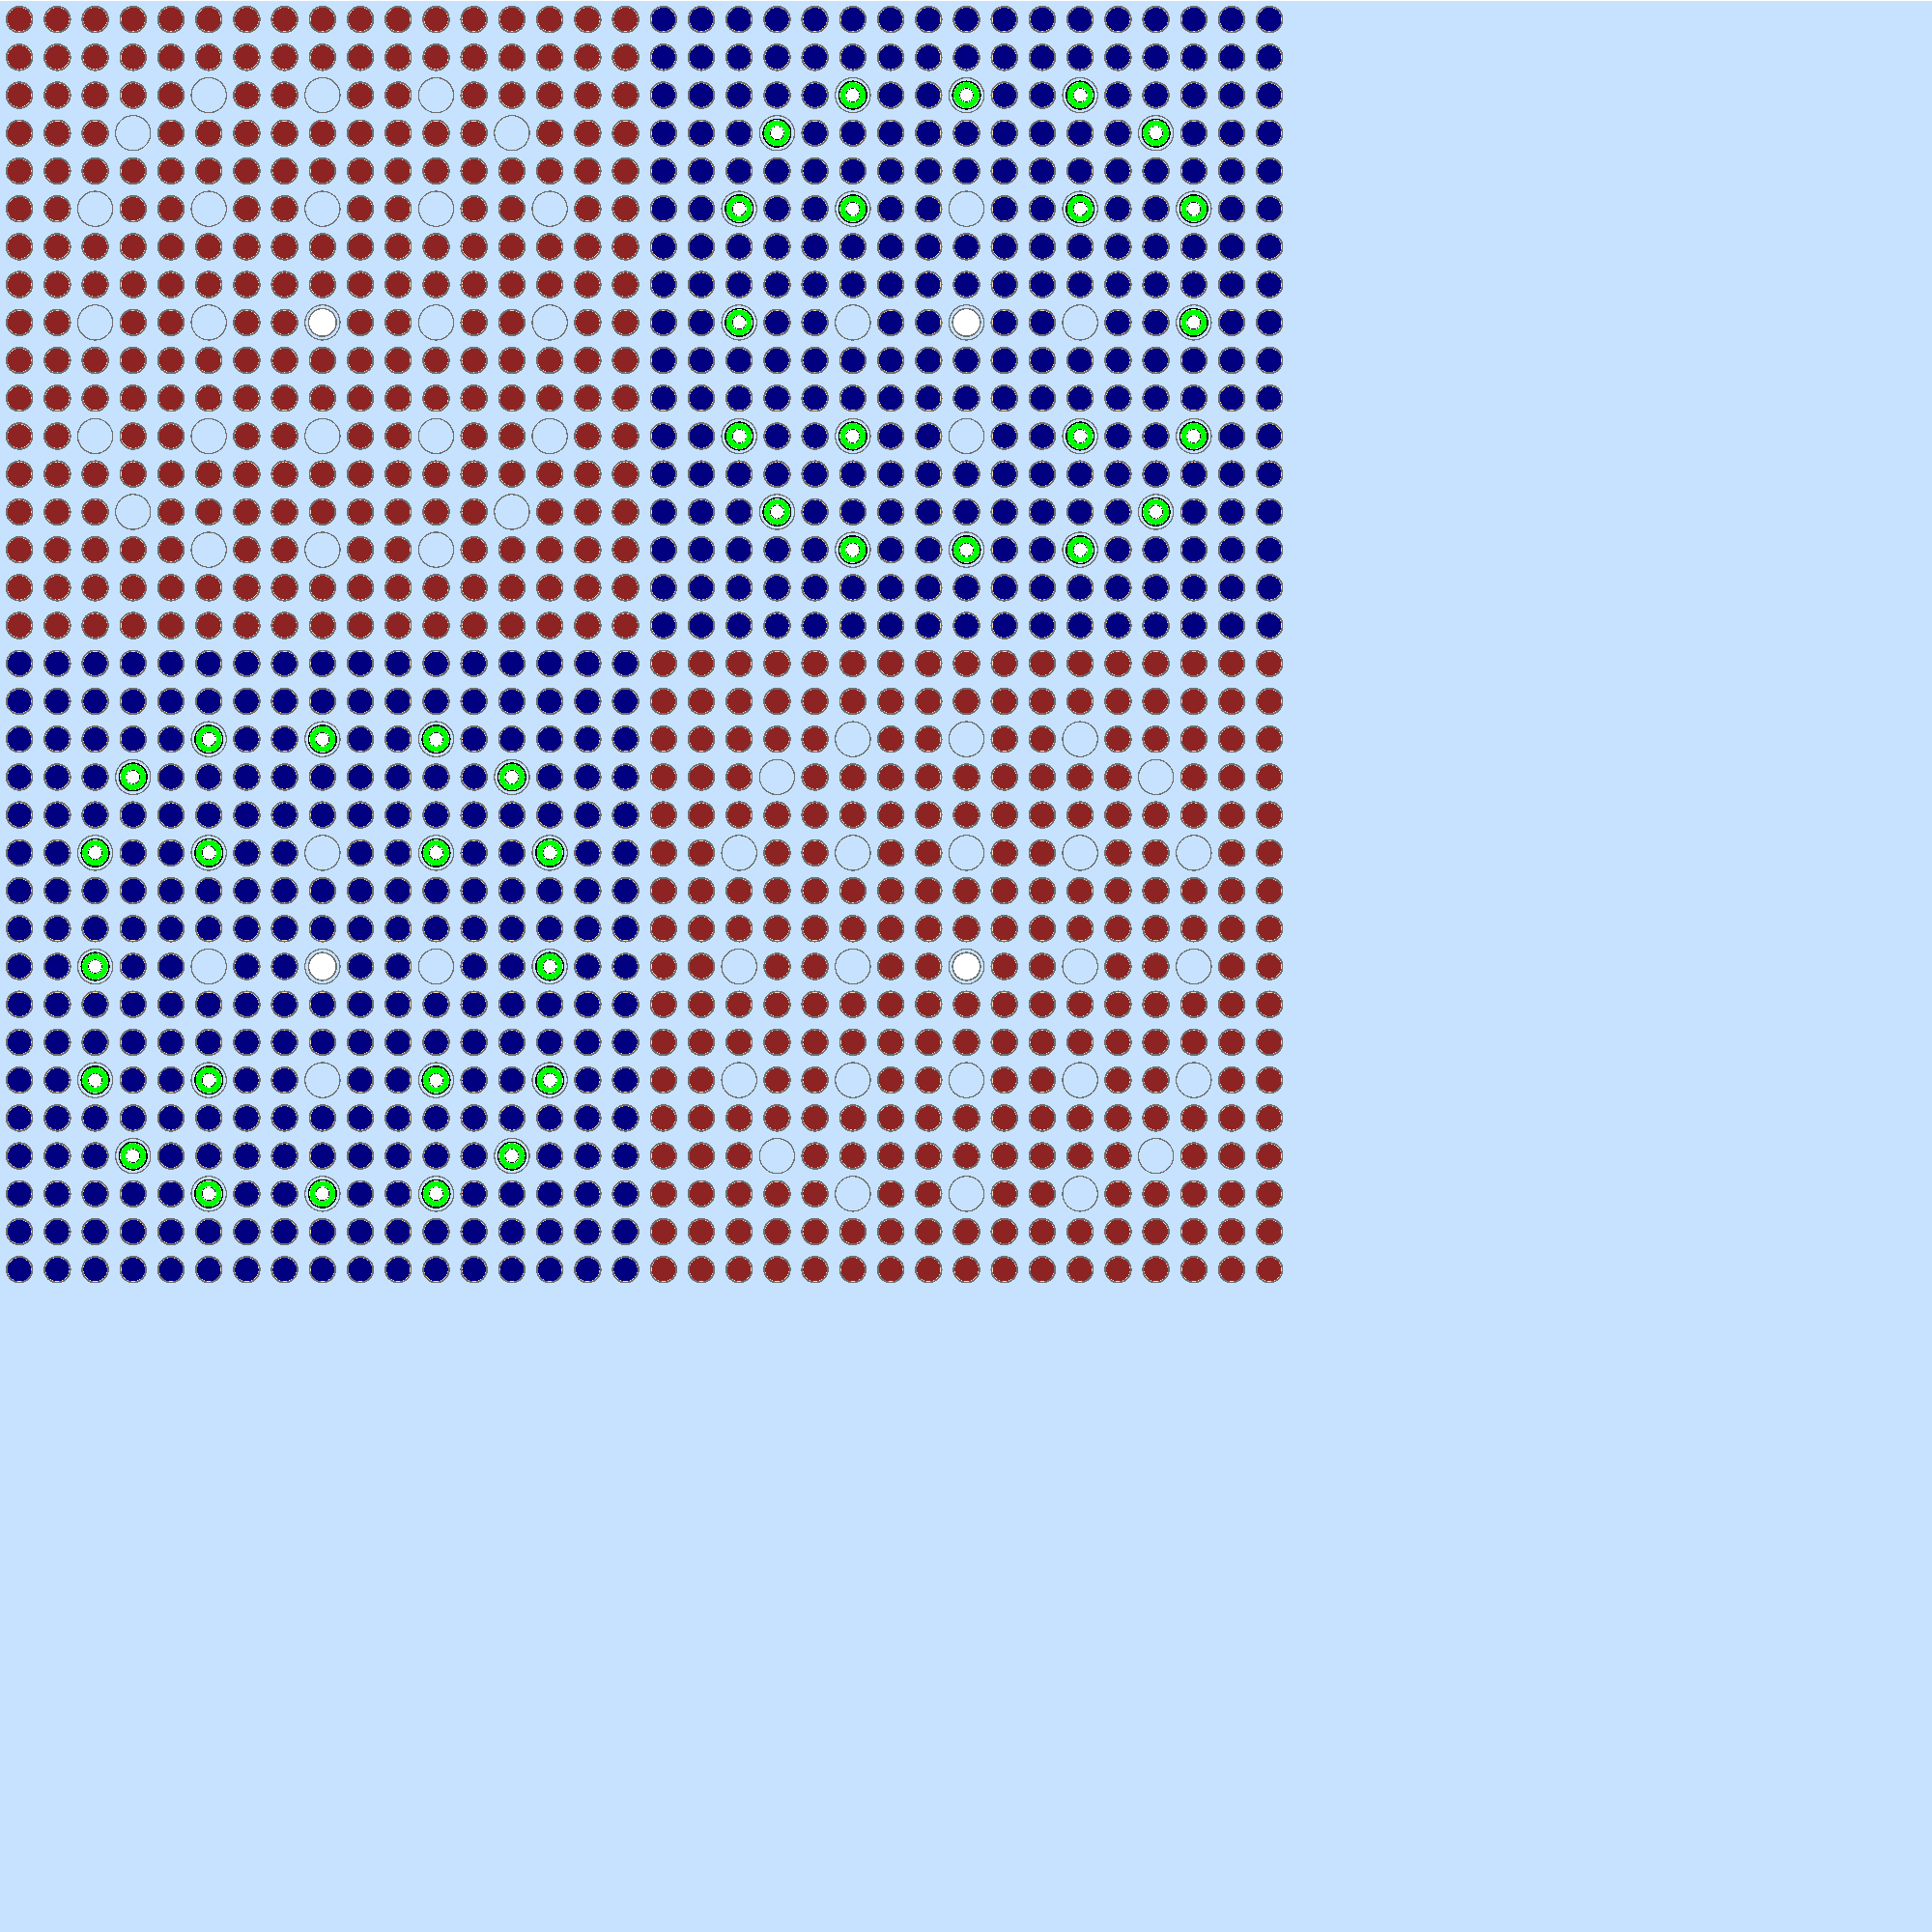
\includegraphics[width=0.93\linewidth]{figures/benchmarks/reflector}
  \caption{}
  \label{fig:reflector}
\end{subfigure}%
\begin{subfigure}{0.47\textwidth}
  \centering
  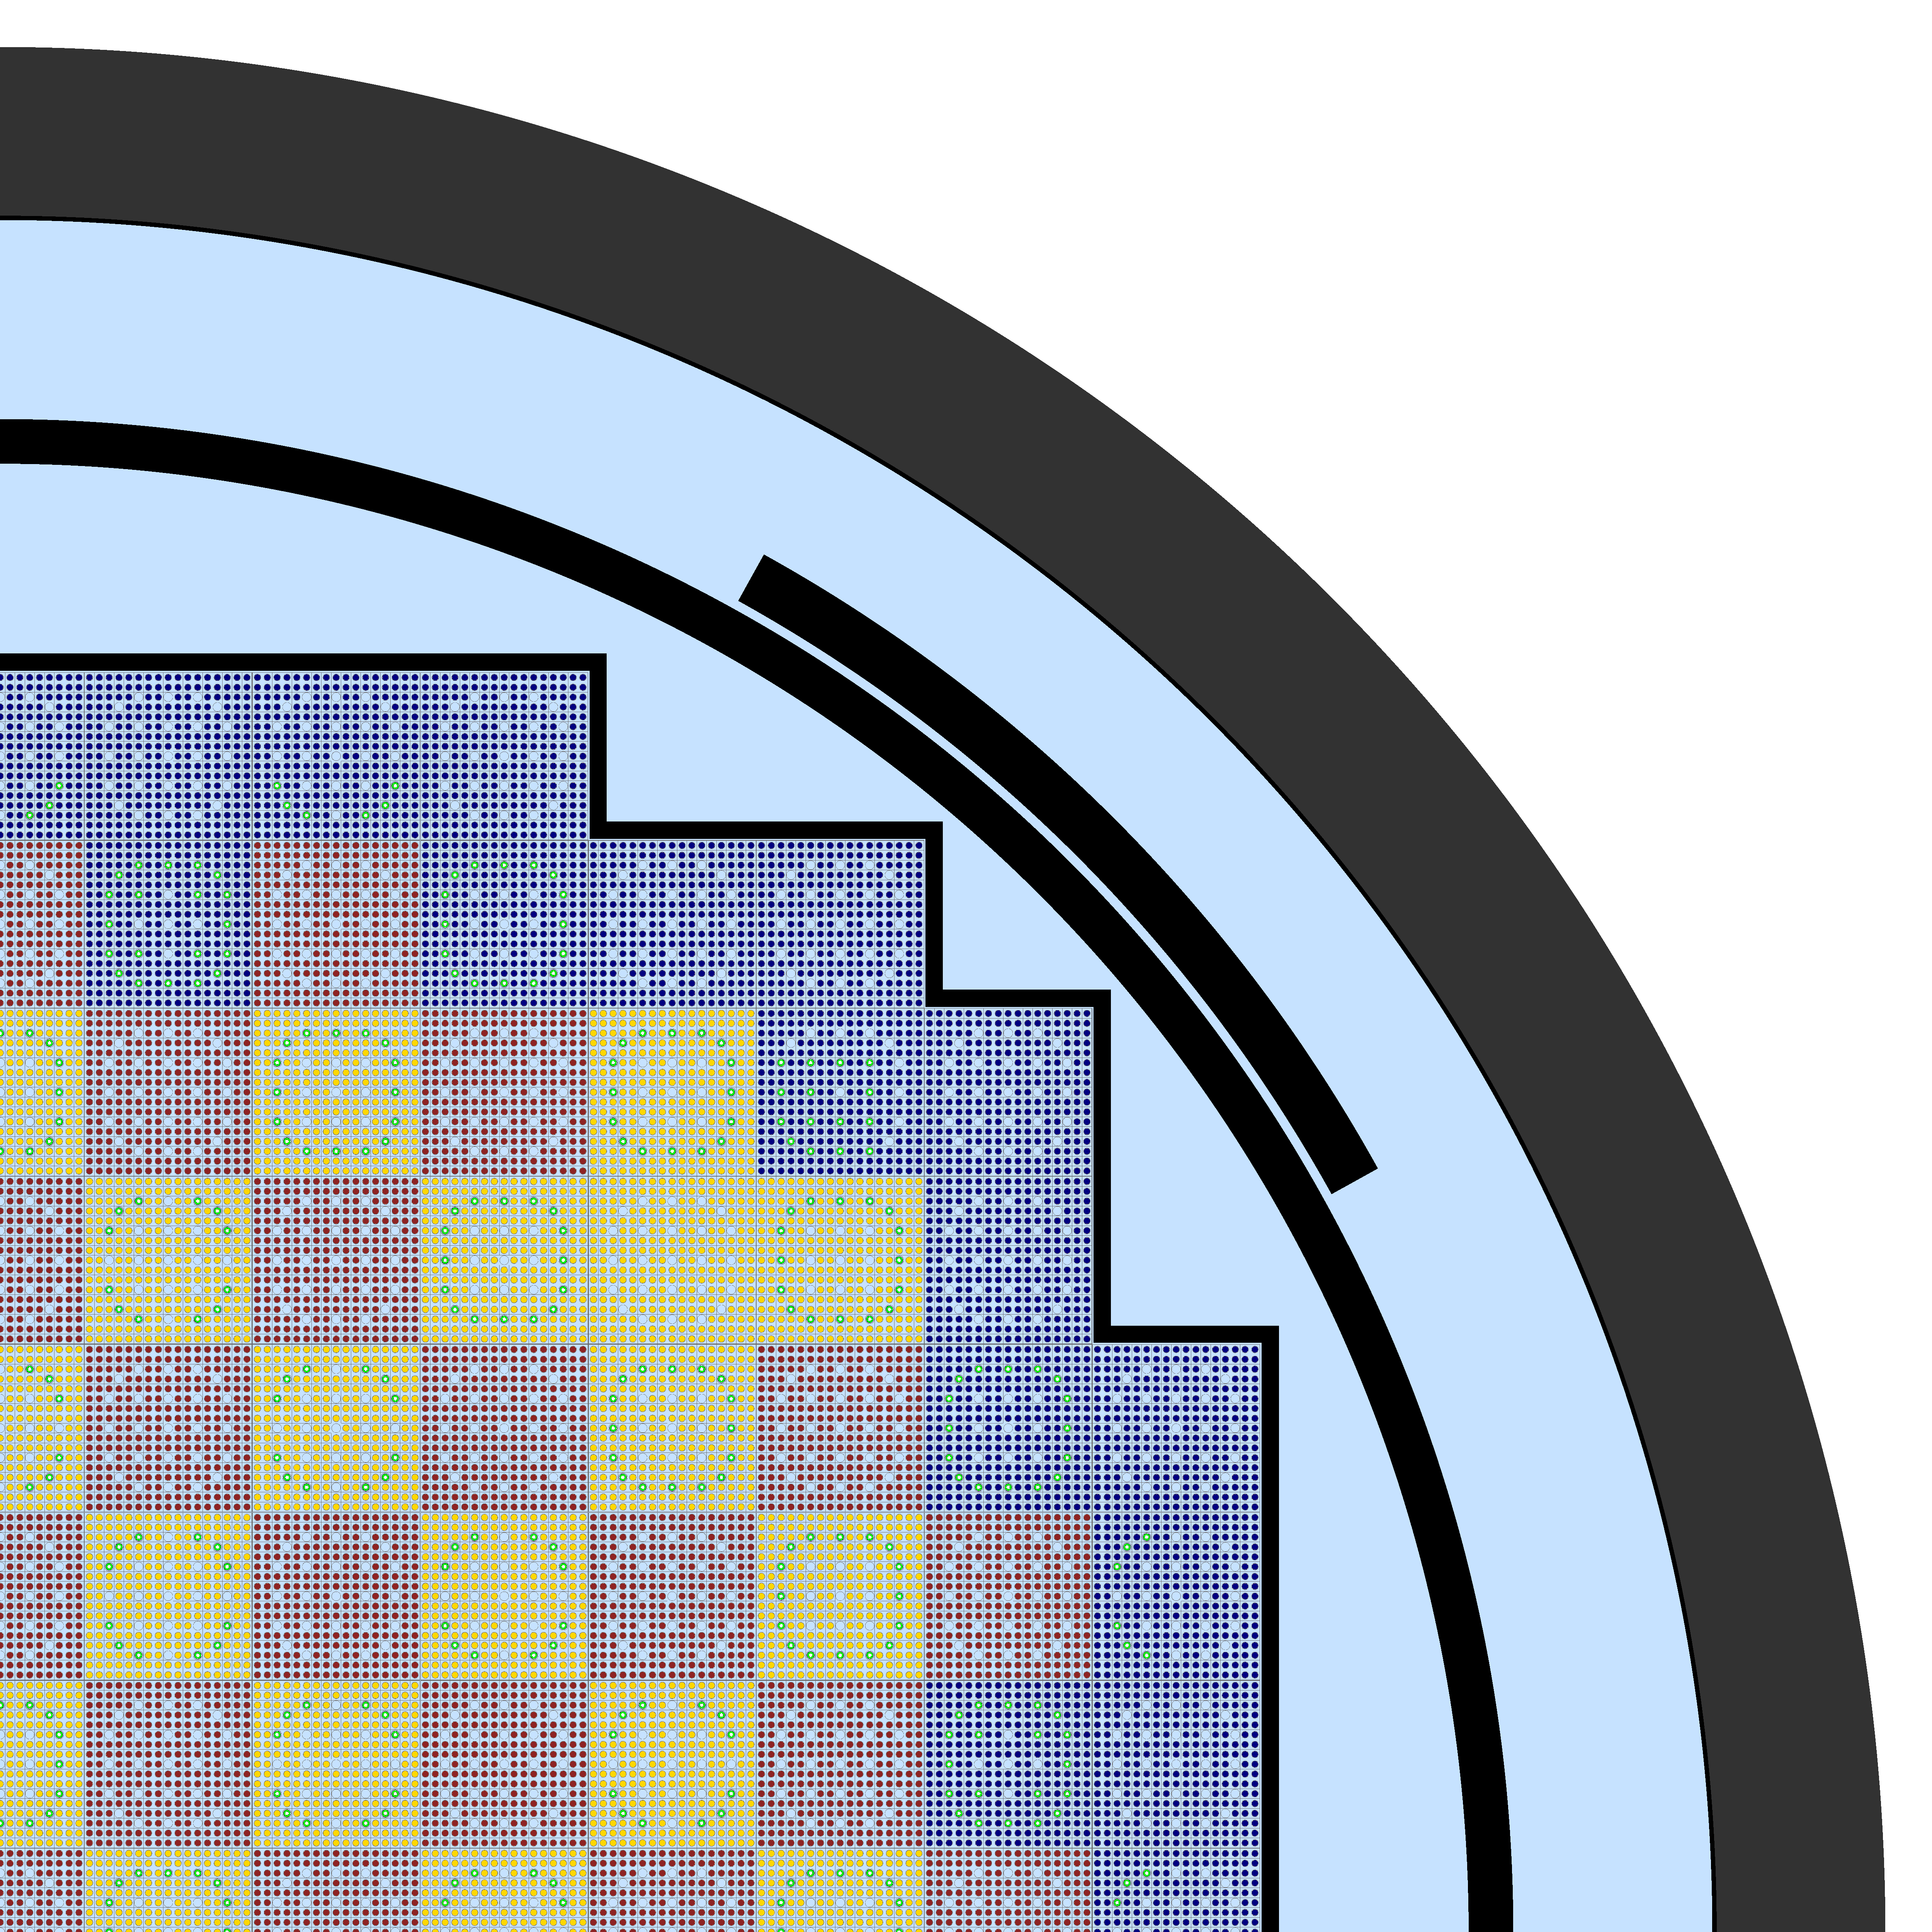
\includegraphics[width=0.93\linewidth]{figures/benchmarks/quarter-core}
  \caption{}
  \label{fig:full-core}
\end{subfigure}
\caption[PWR benchmarks]{The 2$\times$2 colorset with water reflector (a) and the quarter core BEAVRS (b) models used to evaluate the \textit{i}MGXS spatial homogenization scheme.}
\label{fig:benchmarks}
\end{figure}

%%%%%%%%%%%%%%%%%%%%%%%%%%%%%%%%%%%%%%%%%%
\subsection*{Validation Metrics}

-eigenvalues \\
-fission rates \\
-U-238 capture rates \\
-only present U-238 capture rates here \\

\clearpage

%%%%%%%%%%%%%%%%%%%%%%%%%%%
\section*{Results}

%%%%%%%%%%%%%%%%%%%%%%%%%%%%%%%%%%%%%%%%%%%%%%%%%
\subsection*{\textit{i}MGXS Clustered Geometries}

\begin{figure}[h!]
\centering
\begin{subfigure}{0.47\textwidth}
  \centering
  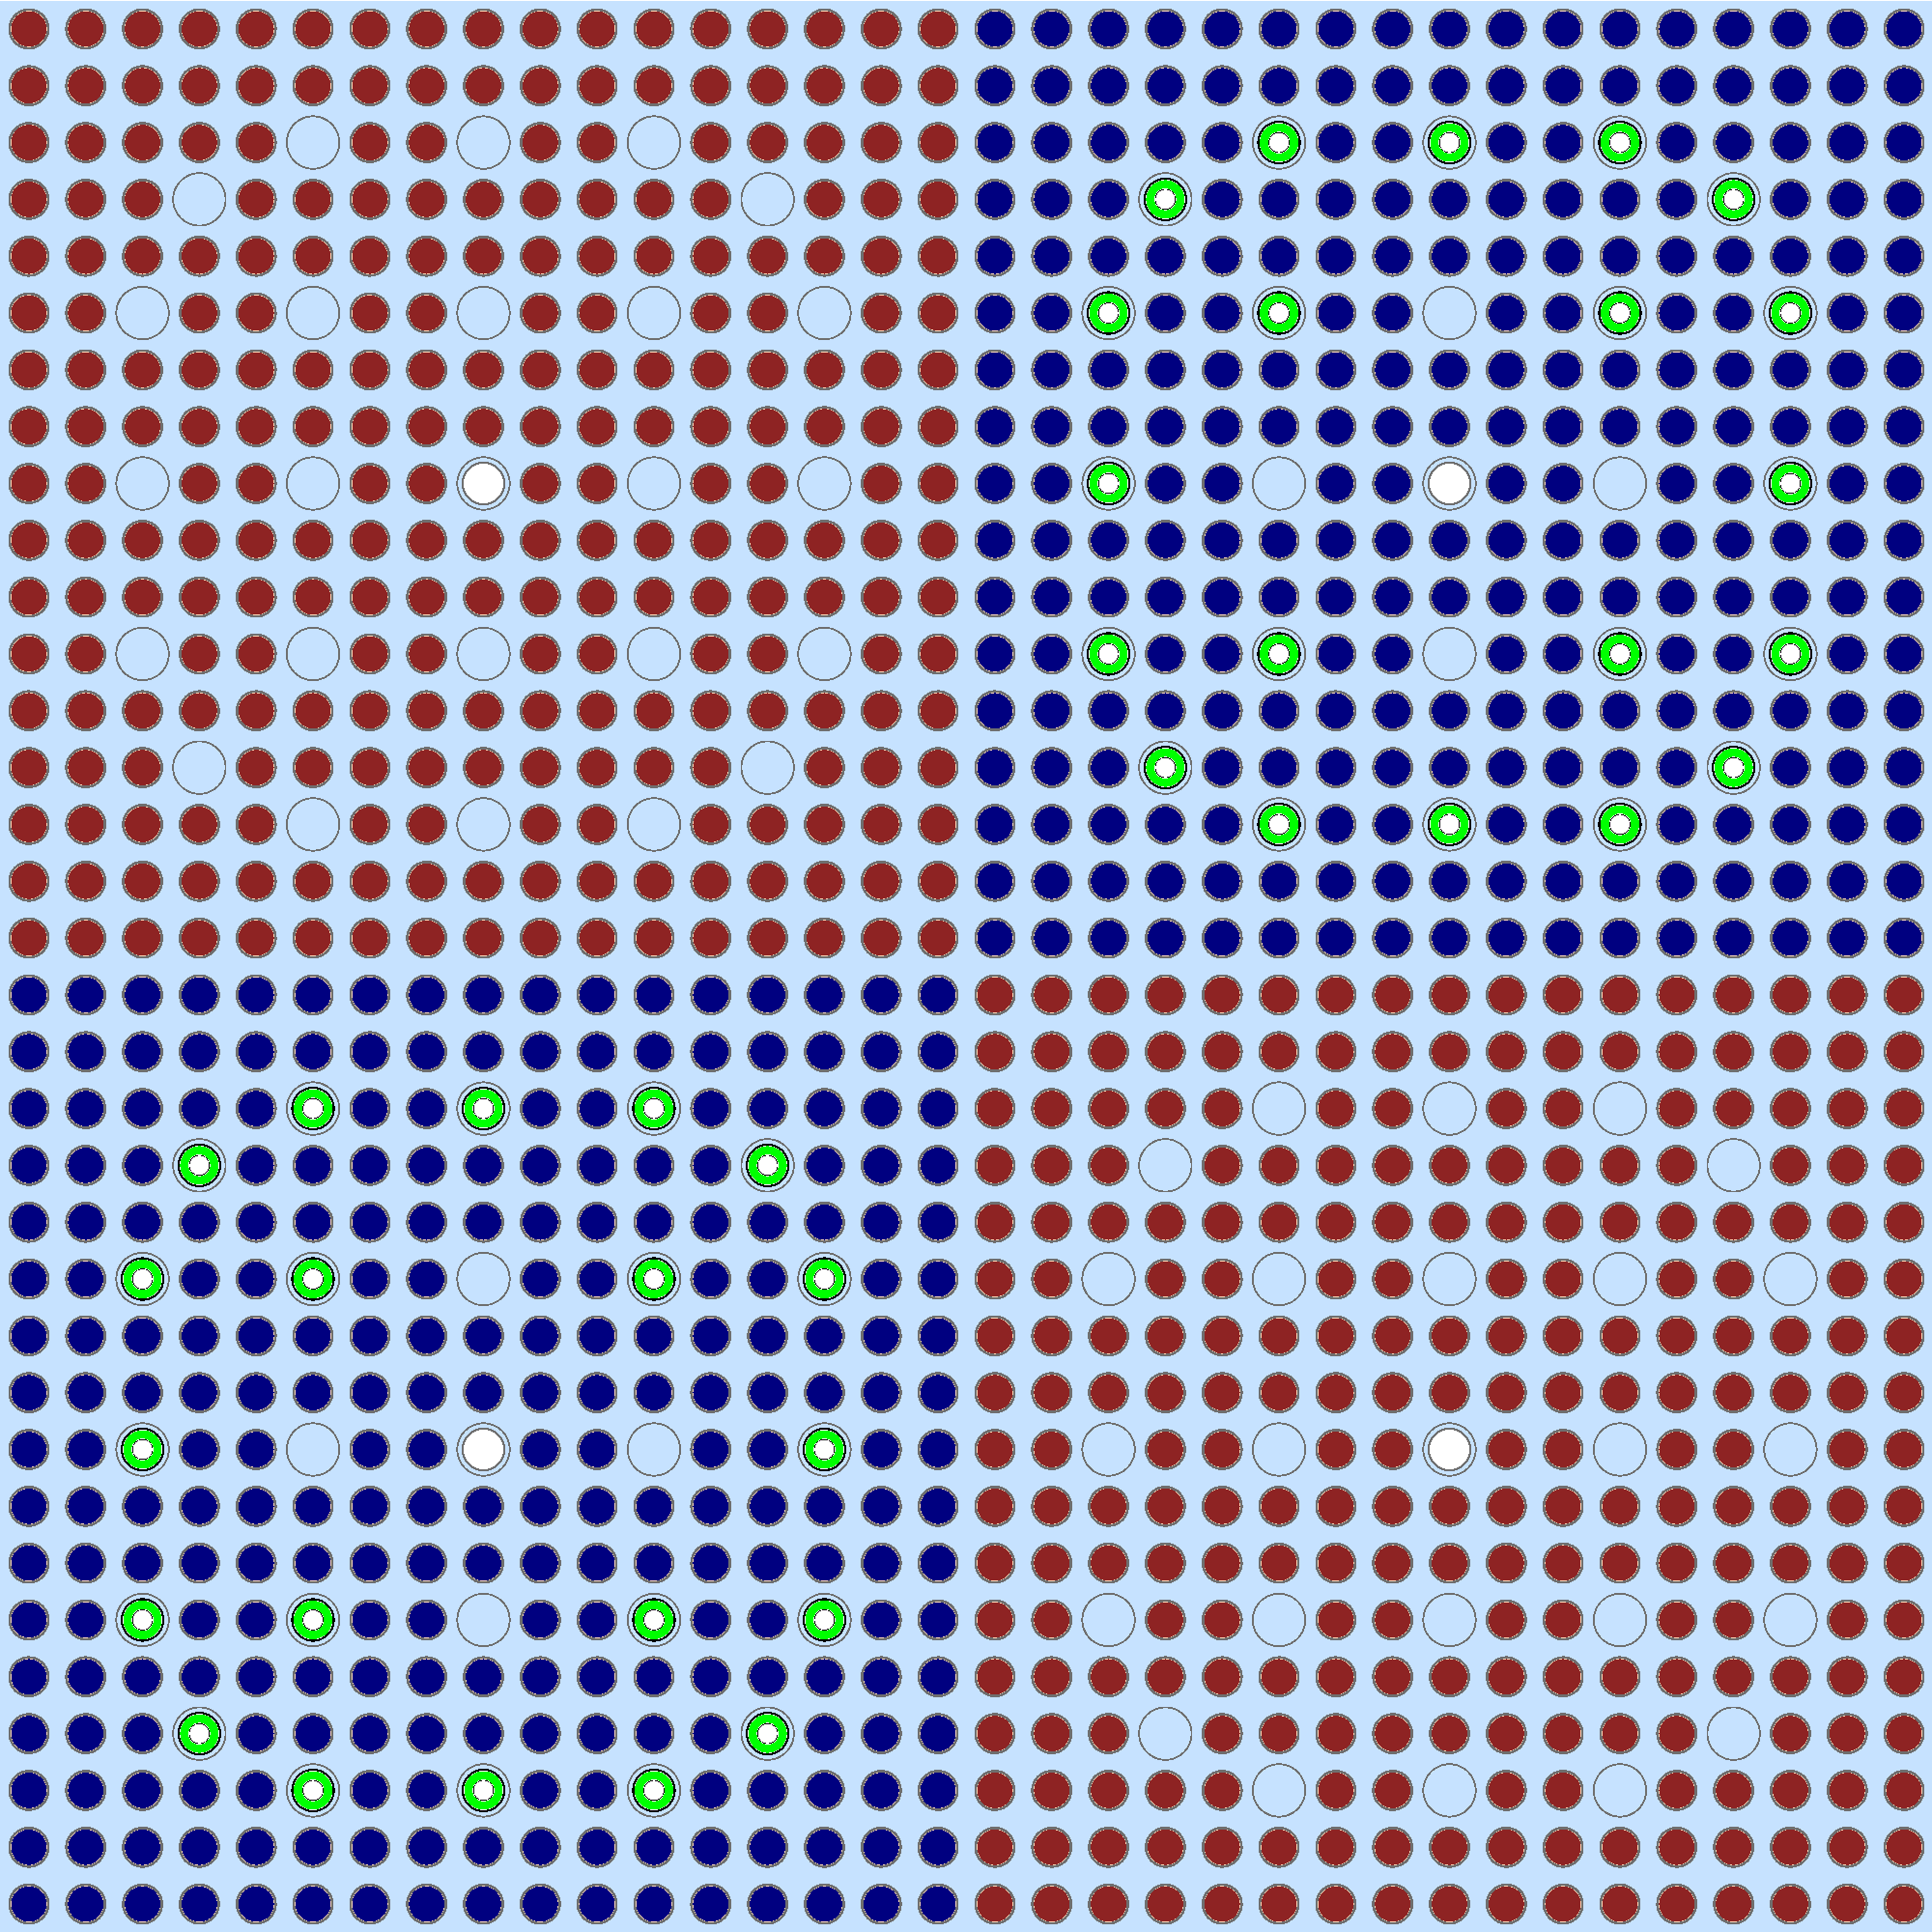
\includegraphics[width=0.95\linewidth]{figures/benchmarks/2x2}
  \caption{}
  \label{fig:reflector}
\end{subfigure}%
\begin{subfigure}{0.47\textwidth}
  \centering
  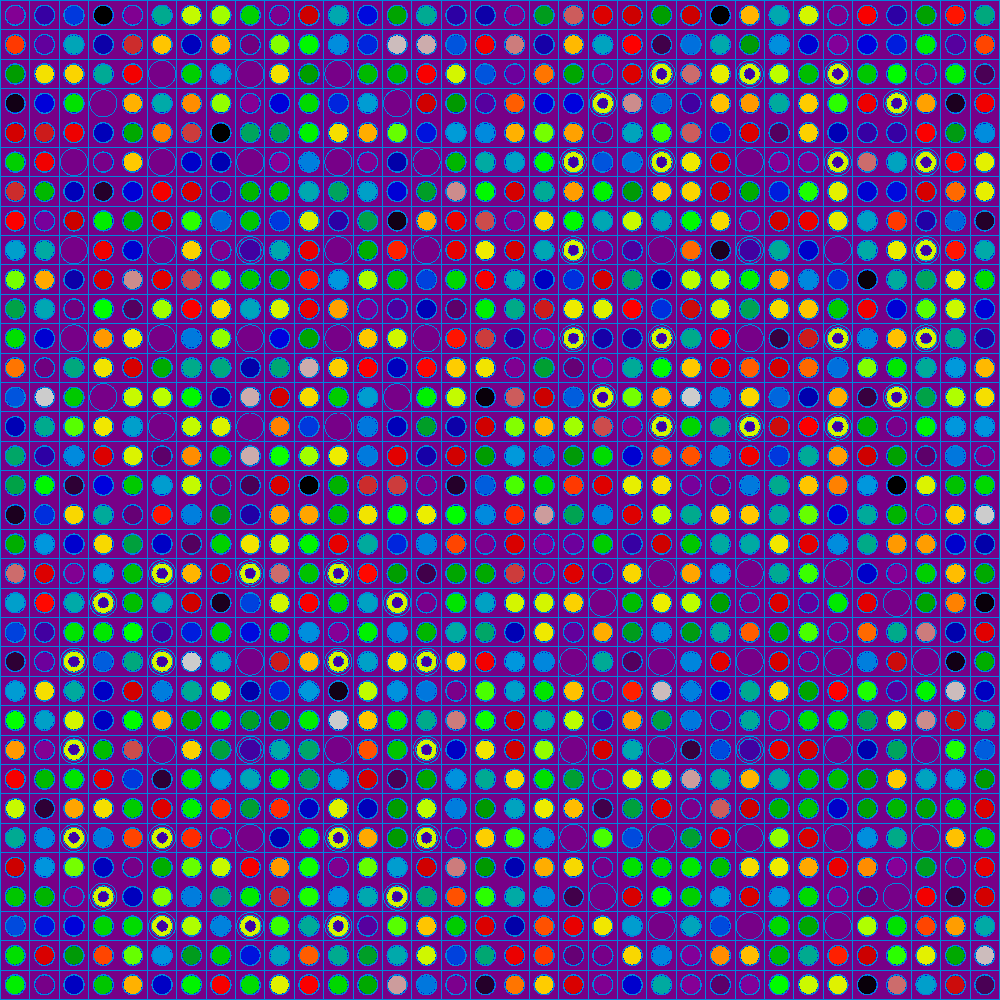
\includegraphics[width=0.95\linewidth]{figures/quantification/homogenization/2x2-degenerate-materials}
  \caption{}
  \label{fig:reflector-degenerate}
\end{subfigure}
\begin{subfigure}{0.47\textwidth}
  \centering
  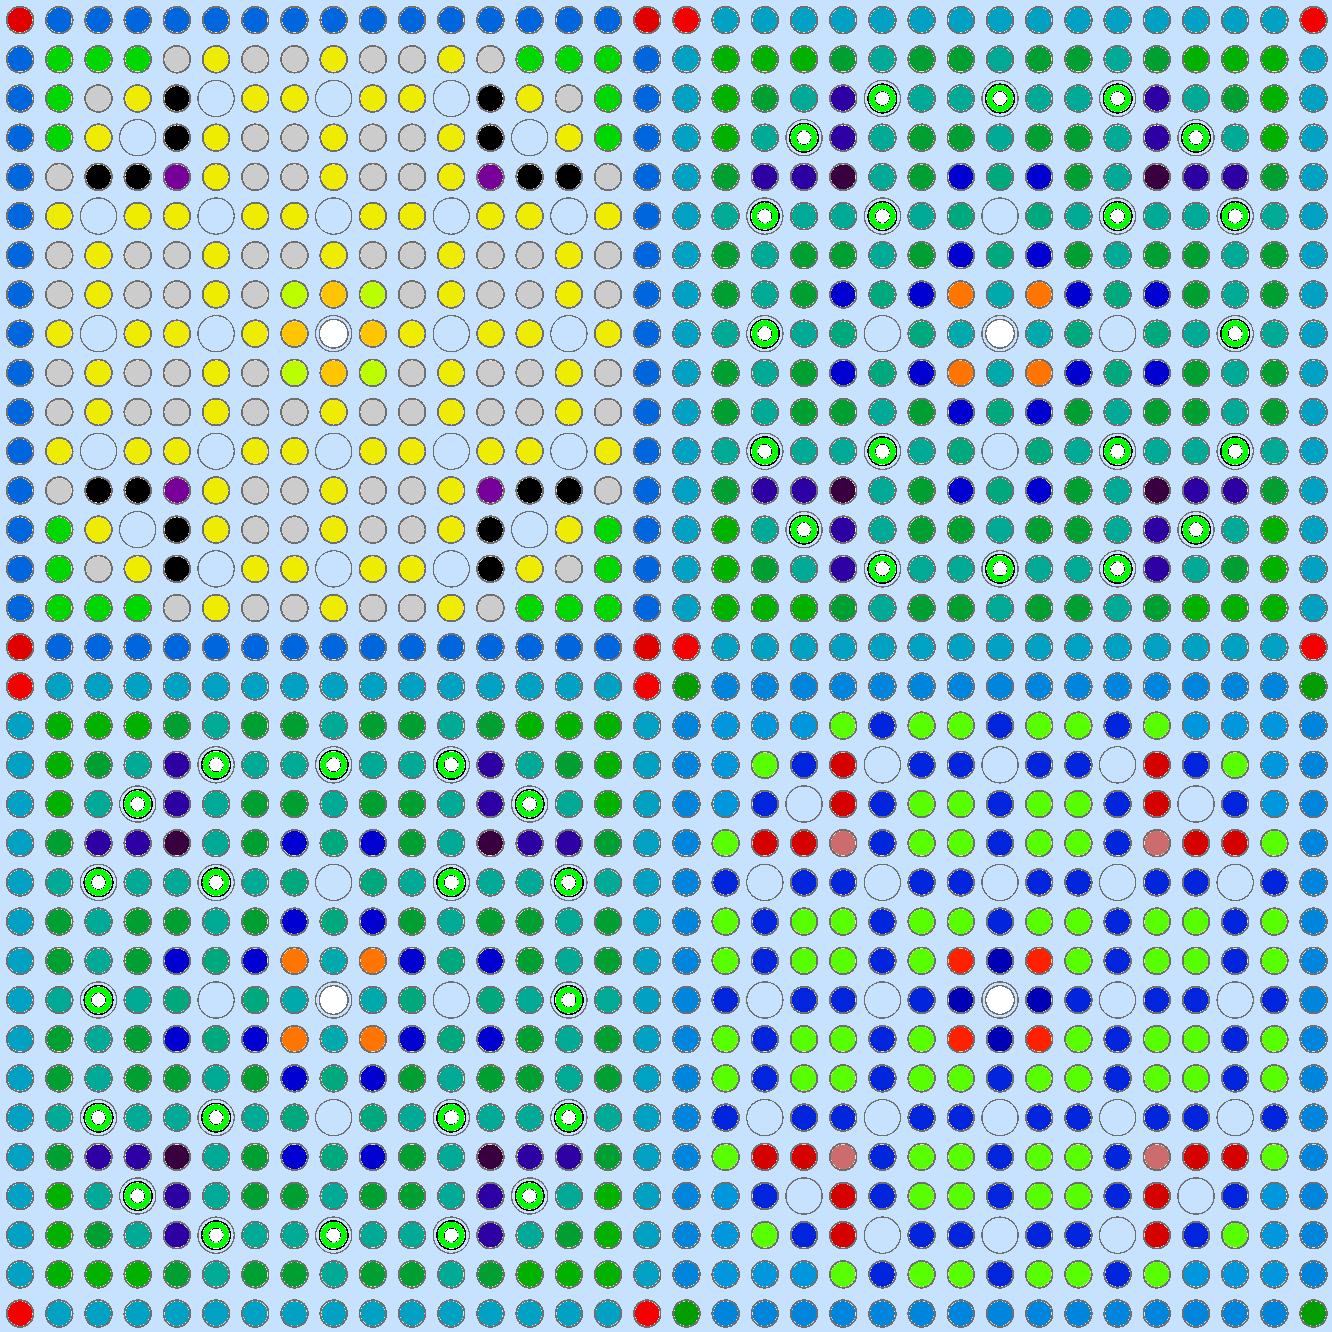
\includegraphics[width=0.95\linewidth]{figures/patterns/lns/reflector/materials}
  \caption{}
  \label{fig:reflector-lns}
\end{subfigure}%
\begin{subfigure}{0.47\textwidth}
  \centering
  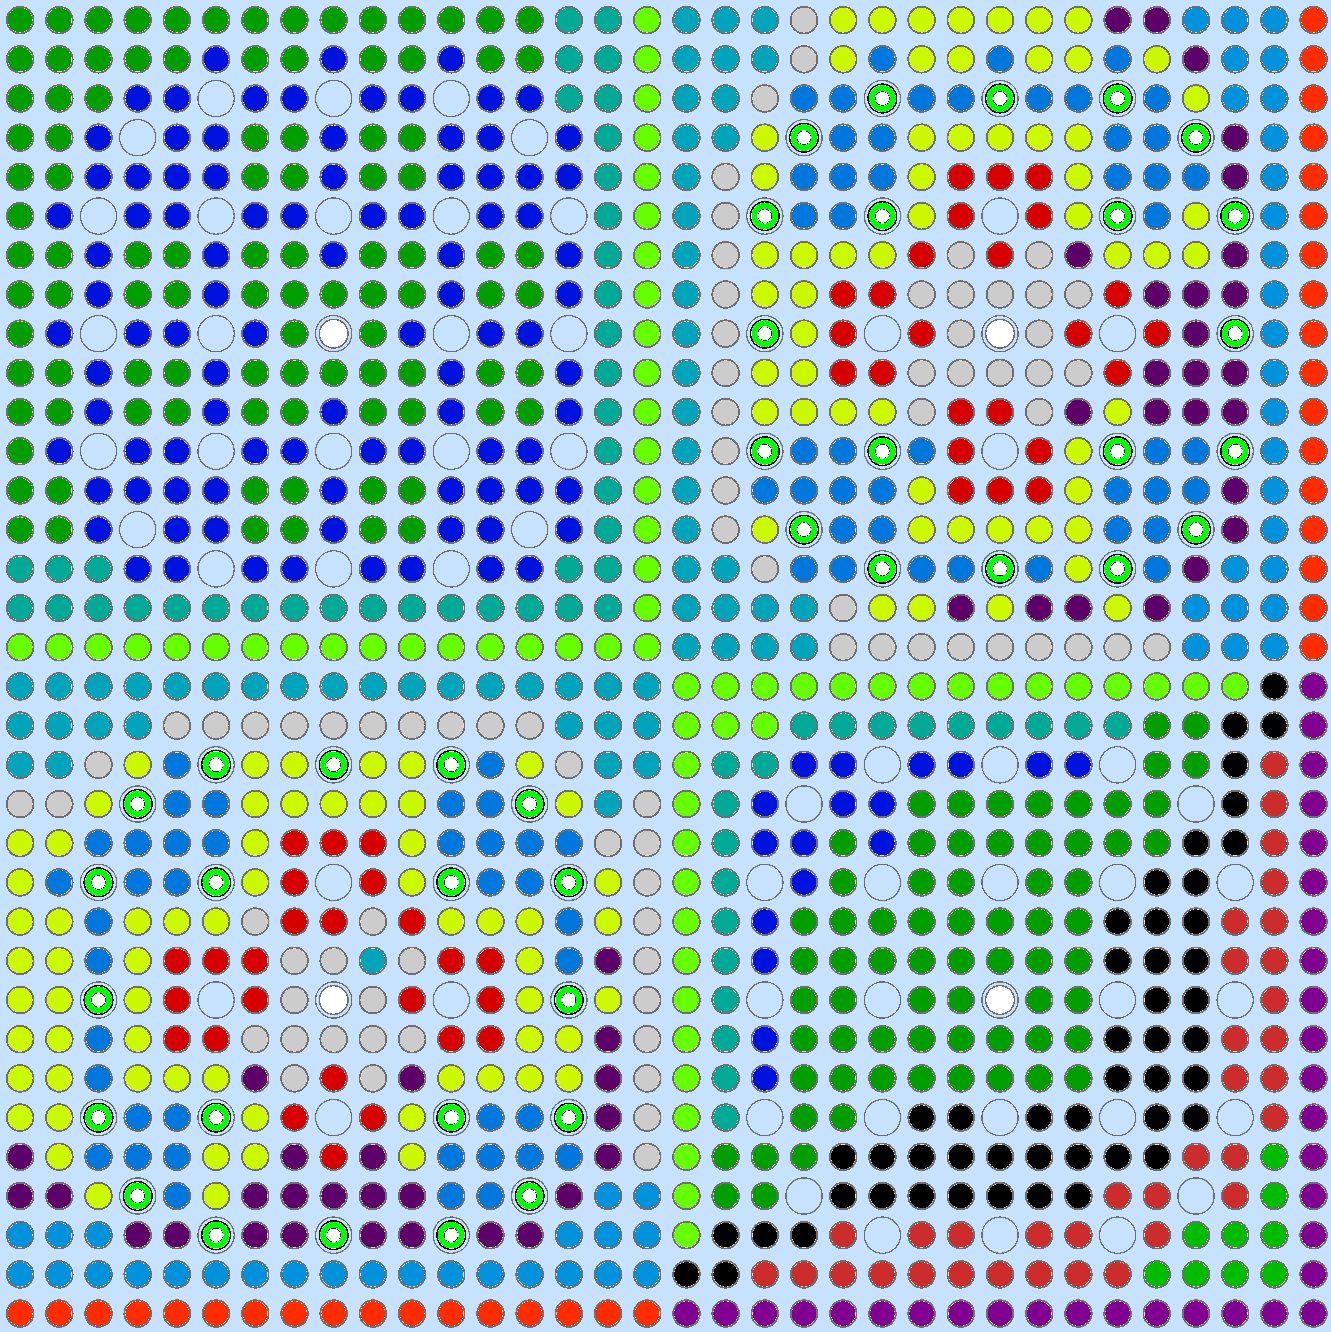
\includegraphics[width=0.95\linewidth]{figures/unsupervised/geometries/with-features/8-clusters/combined/reflector}
  \caption{}
  \label{fig:reflector-8-clusters}
\end{subfigure}
\caption[Materials for the 2$\times$2 colorset]{The materials for the 2$\times$2 colorset with null (a), degenerate (b), LNS (c) and \textit{i}MGXS spatial homogenization with 8 GMM clusters (d).}
\label{fig:colorset-geometries}
\end{figure}

\clearpage

\begin{figure}[h!]
\centering
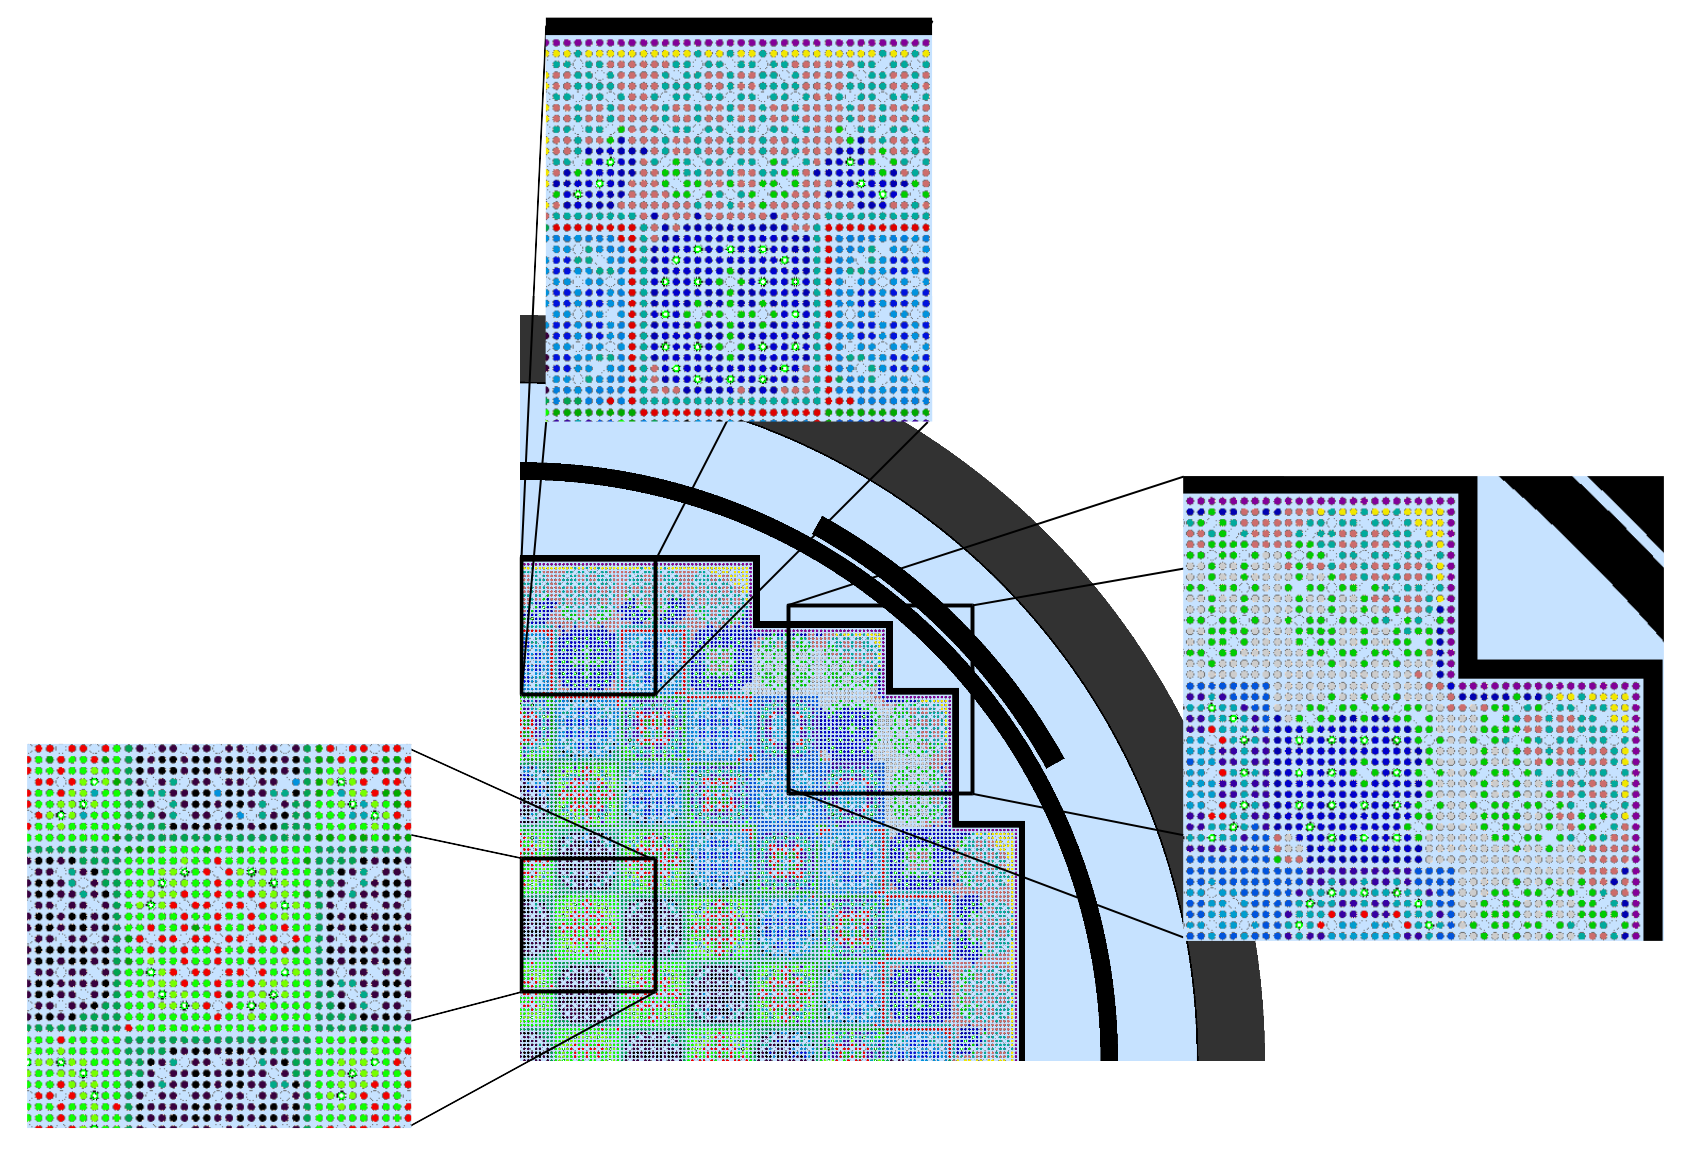
\includegraphics[width=\linewidth]{figures/unsupervised/geometries/with-features/8-clusters/combined/full-core-zoom}
\caption[Materials for the BEAVRS]{The quarter core BEAVRS model with \textit{i}MGXS spatial homogenization.}
\label{fig:full-core-8-clusters}
\end{figure}

%%%%%%%%%%%%%%%%%%%%%%%%%
\subsection*{Eigenvalues}

\begin{table}[ht!]
  \centering
  \caption[OpenMOC eigenvalue bias]{OpenMOC eigenvalue bias $\Delta\rho$ for \textit{i}MGXS spatial homogenization.}
  \small
  \label{table:eigenvalues}
  \vspace{6pt}
  \begin{tabular}{p{4cm} R{0.9cm} R{0.9cm} R{0.9cm} R{0.9cm} R{0.9cm} R{0.9cm}}
  \toprule
  & \multicolumn{6}{S[table-format=6.1]}{\textbf{\# Clusters}} \\
  \cline{2-7}
  \multirow{-2}{*}{\bf Benchmark} &
  \multicolumn{1}{c}{\textbf{1}} & 
  \multicolumn{1}{c}{\textbf{2}} & 
  \multicolumn{1}{c}{\textbf{4}} & 
  \multicolumn{1}{c}{\textbf{8}} & 
  \multicolumn{1}{c}{\textbf{16}} & 
  \multicolumn{1}{c}{\textbf{\# pins}} \\
  \midrule
Colorset w/ Reflector & -141 & -136 & -136 & -134 & -129 & -141 \\
  \midrule
BEAVRS Quarter Core & -122 & -119 & -120 & -119 & -119 & -116 \\
  \bottomrule
\end{tabular}
\end{table}

%%%%%%%%%%%%%%%%%%%%%%%%%%%%%%%%%%%%%%%%%%%%%%%%
\subsection*{Pin-Wise U-238 Capture Rates}

\begin{figure}[h!]
\centering
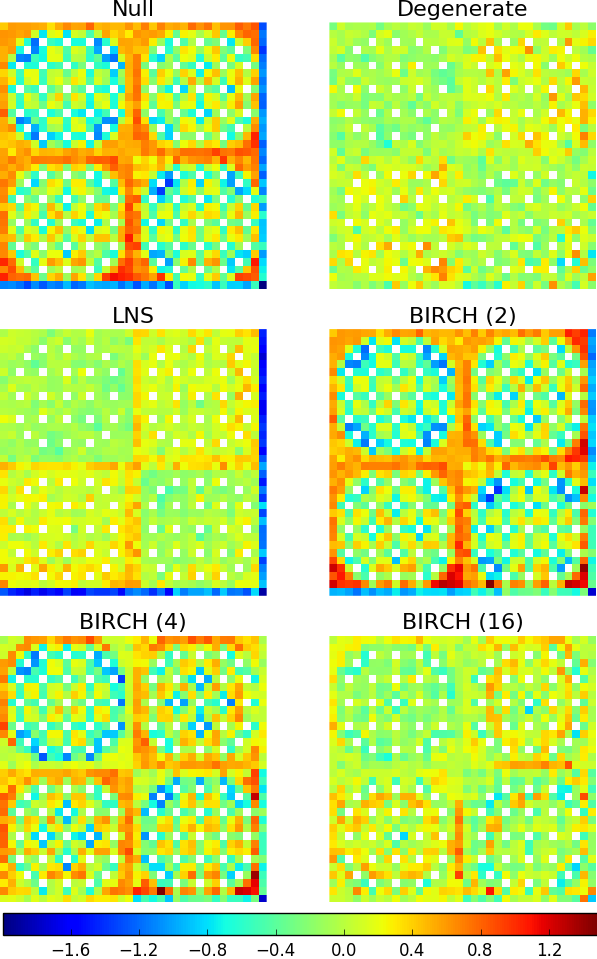
\includegraphics[width=0.83\linewidth]{figures/results/spatial/reflector/capt-err}
\vspace{2mm}
\caption[U-238 capture rate errors for the 2$\times$2 colorset]{U-238 capture rate percentage relative errors for the 2$\times$2 colorset with null, degenerate, LNS and \textit{i}MGXS spatial homogenization with 2, 8 and 16 clusters.}
\label{fig:refl-capt-err}
\end{figure}

\clearpage

\begin{figure}[h!]
\centering
\begin{subfigure}{0.9\textwidth}
  \centering
  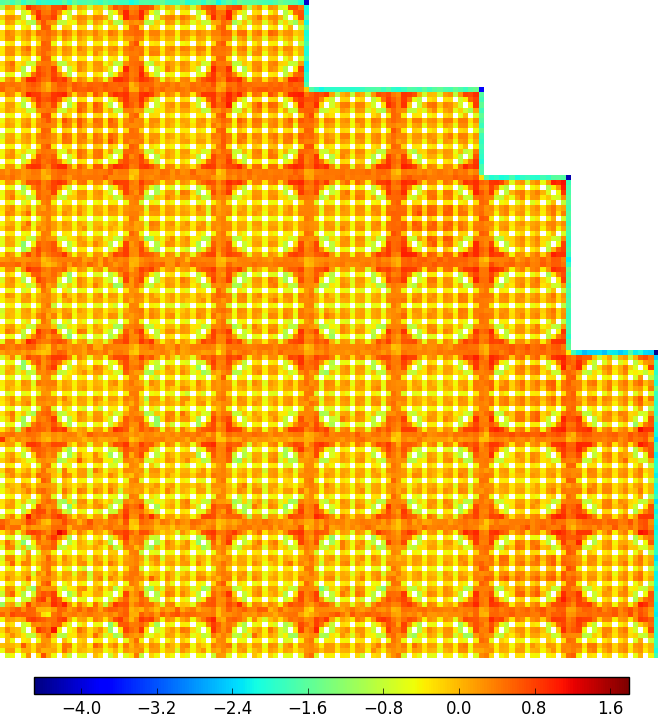
\includegraphics[width=0.65\linewidth]{figures/results/capt-to-fiss/spatial/full-core/capt-to-fiss-err-null}
  \caption{}
  \label{fig:chap11-full-core-capt-err-null}
\end{subfigure}
\begin{subfigure}{0.9\textwidth}
  \centering
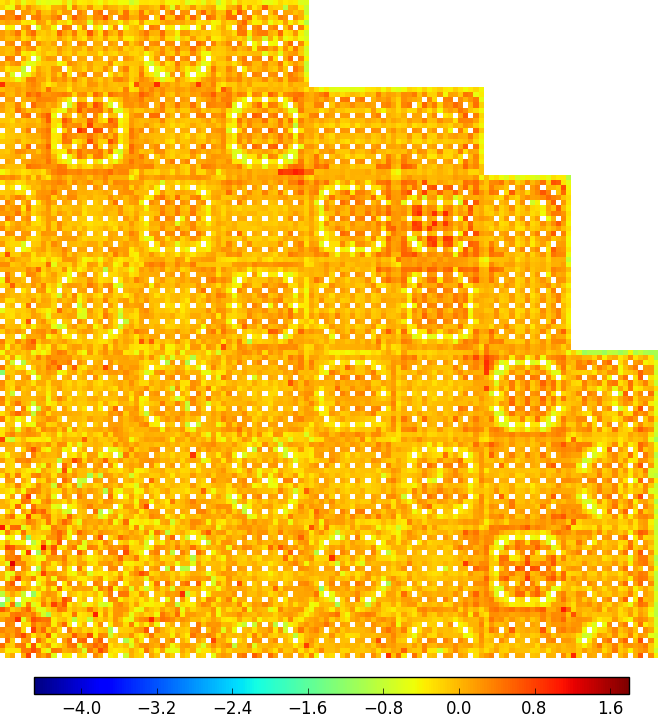
\includegraphics[width=0.65\linewidth]{figures/results/capt-to-fiss/spatial/full-core/capt-to-fiss-err-birch-40}
  \caption{}
  \label{fig:chap11-full-core-capt-err-birch-40}
\end{subfigure}
\caption[U-238 capture rate errors for BEAVRS]{U-238 capture percent relative errors for the quarter core BEAVRS model with null homogenization (a) and \textit{i}MGXS homogenization with 20 clusters (b).}
\label{fig:chap11-full-core-capt-err-b}
\end{figure}

\clearpage

\begin{figure}[h!]
\centering
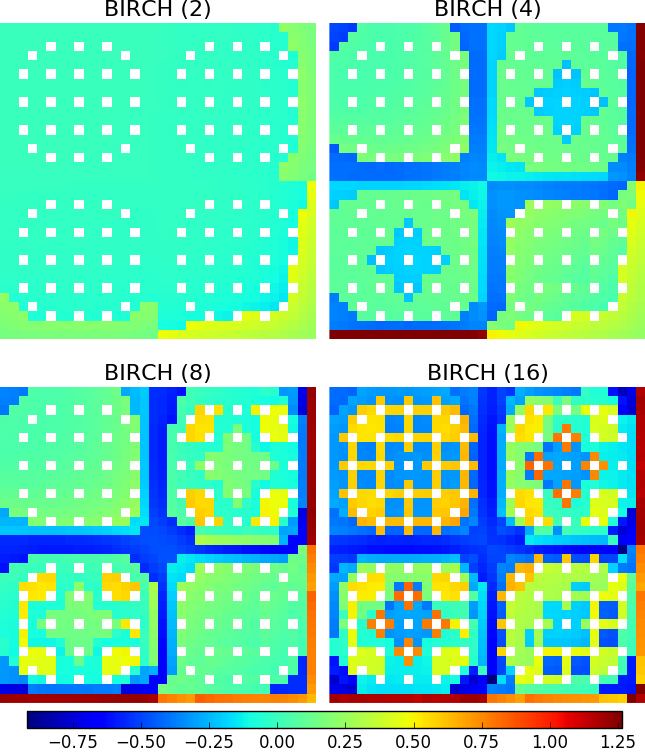
\includegraphics[width=0.85\linewidth]{figures/results/compare/reflector/compare-capt}
\caption[U-238 capture rate comparison for the colorset]{A comparison of U-238 capture rate spatial distributions for \textit{i}MGXS with GMM clustering and null spatial homogenization schemes for the 2$\times$2 colorset.}
\label{fig:refl-capt-rates-comp}
\end{figure}

\clearpage

%%%%%%%%%%%%%%%%%%%%%%%%%%%%%%%%%%%%%%%%%%%%%%%%
\subsection*{Convergence Rates of MOC Solutions}

\begin{figure}[h!]
\centering
\begin{subfigure}{\textwidth}
  \centering
  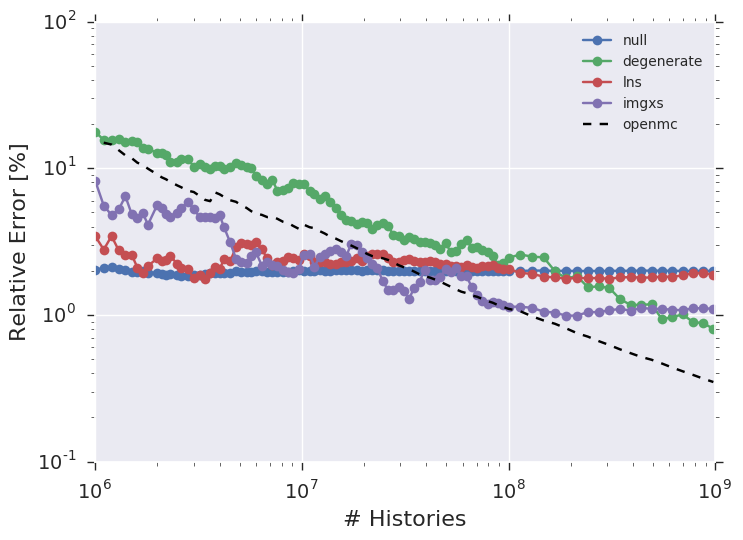
\includegraphics[width=0.9\linewidth]{figures/results/convergence/reflector/max-capt-err-evo-exec-summary}
  \caption{}
  \label{fig:refl-max-converge}
\end{subfigure}
\begin{subfigure}{\textwidth}
  \centering
  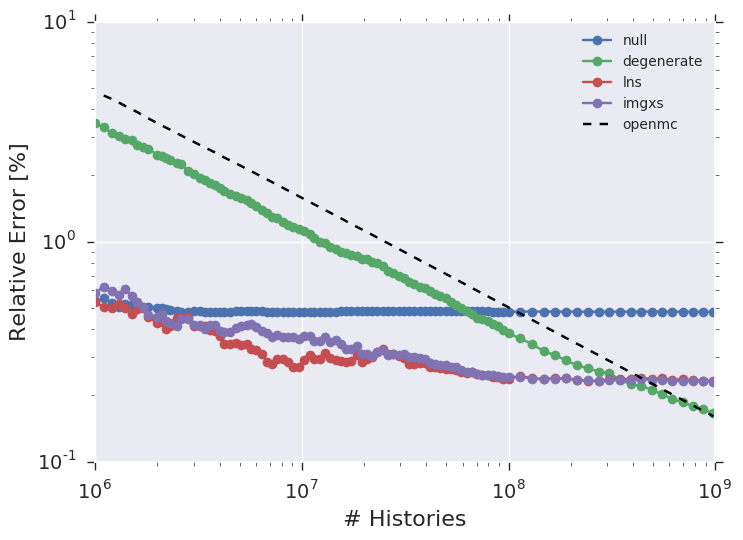
\includegraphics[width=0.9\linewidth]{figures/results/convergence/reflector/mean-capt-err-evo-exec-summary}
  \caption{}
  \label{fig:refl-mean-converge}
\end{subfigure}
\vspace{2mm}
\caption[Fission rate covergence for the 2$\times$2 colorset]{Convergence of the max (a) and mean (b) absolute U-238 capture rate percent relative errors for the 2$\times$2 colorset.}
\label{fig:refl-capture-converge}
\end{figure}

\clearpage

%%%%%%%%%%%%%%%%%%%%%%%%%%%%%%%%%%%%%%%%%%%%%%%%%%%%%%%%%%%%%%%%%%%%%%%%%%%%%%%%
\section*{Conclusions}

%%%%%%%%%%%%%%%%%%%%%%%%%%%%%%%%%%%%%%%%
\subsection*{Contributions to the Field}

-tightly coupled framework for MC and MOC for MGXS \\
-useful for both MGXS generation as well as validation of MOC \\
-identified fundamental issue with flux separability approx. and 

%%%%%%%%%%%%%%%%%%%%%%%%%
\subsection*{Future Work}

-speed up OpenMOC full core: \\
  -find a way use quarter assembly CMFD mesh \\
  -linear source to reduce number of spatial zones \\
  -vectorize transport solver over energy groups \\

evaluate \textit{i}MGXS scheme:
-add anisotropic scattering to OpenMOC to enable solution of the ``correct'' problem
-systematic study of featues -- ones actually matter? \\
-systematic study to understand impact of dimensionality reduction \\
-systematic study to understand impact of clustering algorithms \\
-more research into model selection schemes -- none of them robustly works for my case studies! \\
-evaluate \textit{i}MGXS with clustering ``on-the-fly'' with noisy MC tally data \\
-can \textit{i}MGXS reduce the number of necessary energy groups?? \\

reach goals:\\
-multi-physics applications: moderator density, fuel temperature, burnup, etc. as features \\
-machine learning to optimize energy group structures \\


%%%%%%%%%%%%%%%%%%%%%%%%%%%%%%%%%%%%%%%%%%%%%%%%%%%%%%%%%%%%%%%%%%%%%%%%%%%%%%%%
%%%%%%%%%%%%%%%%%%%%%%%%%%%%%%%%%%%%%%%%%%%%%%%%%%%%%%%%%%%%%%%%%%%%%%%%%%%%%%%%
% BIBLIOGRAPHY

\begin{singlespace}
\bibliographystyle{ans}
\bibliography{references}
\end{singlespace}

\end{document}
